\documentclass[%
    school=etsisi,%
    type=pfg,%
    degree=61IW,%
    authorsex=m,%
    directorsex=m,%
]{upm-report}

\usepackage{wrapfig}

\addbibresource{references.bib}

\author{Marcos Martínez Francisco}
\title{AI-nance:~Stocks~Prediction}
\director{Alberto Díaz Álvarez}

\abstract{spanish}{
  Predecir el precio de acciones como un método de inversión presenta un alto nivel de complejidad. Es bien conocida la gran capacidad de los ordenadores a la hora de reconocer patrones y la correlación entre la estadística y los mercados financieros, lo que los convierte en un perfecto campo de aplicación. Esta tesis pretende construir la infraestructura y los modelos de predicción necesarios para soportar un servicio de predicción RESTful utilizando algoritmos de deep learning junto a las herramientas de orquestación y contenedorización adecuadas.
   
  Para probar la hipótesis de que los precios de las acciones no pueden predecirse con precisión basándose únicamente en su historia pasada, se han aplicado múltiples técnicas de predicción. Se ha construido una infraestructura completa utilizando un patrón de microservicios, centrándose en la automatización y el despliegue, y se alimentó todo el historial bursatil de Google a los diferentes modelos para evaluar su respectiva precisión. Los resultados se mostraron en la misma línea de lo hipotetizado, ninguno de los modelos ha sido capaz de mostrar altos porcentajes de precisión.
   
  Estos resultados sugieren que las variaciones de los precios son impulsadas por múltiples factores, algunos de los cuales son externos al activo, y por lo tanto no pueden predecirse totalmente unicamente por el precio histórico. Teniendo esto en cuenta, hay que valorar todos los factores del entorno que rodean al activo cuando se intenta generar predicciones en los mercados financieros.

}
\keywords{spanish}{Mercados Financieros; Arquitectura de Microservicios; Docker; CI/CD; Redes LSTM}

\abstract{english}{
   Forecasting stock prices as an investment method presents a high level of complexity. It is well known computer's great capacity at recognizing patterns and the correlation between statistics and financial markets, which makes them a perfect field to apply machine learning algorithms. This thesis aims to build the necessary infrastructure and prediction models to support a \gls{RESTful} prediction service using deep learning algorithms along with the proper orchestration and containerization tools.
   
   To test the hypothesis that stock prices can not be accurately predicted based just on their past history, multiple prediction techniques have been applied. An entire infrastructure has been built using a micro-services pattern, focusing on automation and deployment, and the entire trading history of Google was fed to the different models to evaluate their respective accuracy. The results were along the lines of the hypothesized outcome, as none of the models were able to show high percentages of accuracy.
   
   These results suggest that price variations are driven by multiple factors, some of which are external to the asset, and therefore cannot be entirely predicted just by historical price. Bearing this in mind, all of the environmental factors that surround the asset must be taken into account when trying to generate predictions in financial markets.
}
\keywords{english}{Financial Markets; Micro-services Architecture; \gls{Docker}; CI/CD; LSTM Networks}

\acknowledgements{
   I am deeply indebted to my family, thanks to them I got to where I am today.\\
   I could not have undertaken this journey without Rubén, who has helped me out throughout the entire thesis.\\
   I must also thank my mentor Alberto, for his enormous patience with me.\\
   To all my friends, who have helped me during my low moments and especially to Abby for helping me out with the editing of the thesis.
 }

\begin{document}

\newglossaryentry{maths}{
        name=mathematics,
        description={Mathematics is what mathematicians do}
}

\newglossaryentry{RESTful}{
        name=RESTful,
        description={Architectural style for an application program interface that uses HTTP requests to access and use data}
}

\newglossaryentry{Docker}{
        name=Docker,
        description={Operating system level virtualization to deliver software in packages called containers}
}

\newglossaryentry{Kanban}{
        name=Kanban,
        description={Scheduling system for lean manufacturing}
} 

\newglossaryentry{Django}{
        name=Django,
        description={Python-based web framework}
}

\newglossaryentry{YAML}{
        name=YAML,
        description={Human readable data serialization language}
}

\newacronym{ine}{INE}{Instituto Nacional de Estadística}
\newacronym{pfg}{PFG}{Cambiar a ingles}
\newacronym{tfg}{FDP}{Final Degree Project}
\newacronym{pfm}{PFM}{Proyecto Fin de Máster}
\newacronym{td}{TD}{Tesis Doctoral}
\newacronym{ai}{AI}{Artificial Intelligence}
\newacronym{ml}{ML}{Machine Learning}
\newacronym{sl}{SL}{Supervised Learning}
\newacronym{usl}{UL}{Unsupervised Learning}
\newacronym{dl}{DL}{Deep Learning}
\newacronym{ann}{ANN}{ArtificialNeuronal Network}
\newacronym{gan}{GAN}{Generative Adversarial Network}
\newacronym{rnn}{RNN}{Recurrent Neural Networks}
\newacronym{es}{ES}{Expert System}
\newacronym{nlp}{NLP}{Natural Language Processing}
\newacronym{lstm}{LSTM}{Long Short Term Memory}
\newacronym{cl}{CL}{Computational Linguistics}
\newacronym{ct}{CT}{Control Theory}
\newacronym{cs}{CS}{Cognitive Science}
\newacronym{dt}{DT}{Decision Theory}
\newacronym{etf}{ETF}{Exchange Traded Fund}
\newacronym{st}{ST}{Short Trading}
\newacronym{mdp}{MDP}{Markov Decision Process}
\newacronym{ddpg}{DDPG}{Deep Deterministic Policy Gradient}
\newacronym{dpg}{DPG}{Deep Deterministic Policy Gradient}
\newacronym{vm}{VM}{Virtual Machine}
\newacronym{os}{OS}{Operating System}
\newacronym{fpga}{FPGA}{Field Programmable Gate Arrays}
\newacronym{gpu}{GPU}{Graphics Processing Unit}
\newacronym{soa}{SOA}{Service Oriented Architecture}
\newacronym{api}{API}{Aplication Programming Interface}
\newacronym{dnn}{DNN}{Dense Neural Network}
\newacronym{mlp}{MLP}{Multilayer Perceptron}
\newacronym{cnn}{CNN}{Convolutional Neural Network}
\newacronym{cd}{CD}{Continuous Deployment}
\newacronym{ci}{CI}{Continuous Integration}
\newacronym{iot}{IoT}{Internet of Things}
\newacronym{json}{JSON}{JavaScript Object Notation}
\newacronym{http}{HTTP}{HyperText Transfer Protocol}
\newacronym{grpc}{gRPC}{Google Remote Procedure Calls}

\frontmatter

\begin{KeepFromToc}
  \tableofcontents
\end{KeepFromToc}

\begin{KeepFromToc}
  \listoffigures
\end{KeepFromToc}

\begin{KeepFromToc}
  \lstlistoflistings
\end{KeepFromToc}

\begin{KeepFromToc}
  \listoftables
\end{KeepFromToc}



\mainmatter

\chapter{Introduction}
\label{ch:introduccion}

\gls{ai} is one of the scientific areas that has gained the most popularity over the last decade~\cite{iagoogletrend}. While it is true that \gls{ai} is a relatively new theoretical field created in the mid-twentieth century~\footnote{The term \enquote{Artificial Intelligence} was first coined by John McCarthy in 1956~\cite{definitionIaMcCarthy}.}, it is only now that it has begun to offer real and accurate solutions beyond a purely research-focused framework, as a result of the exponential increase of the availability of colossal data sets as well as monstrous computing power. There is a huge variety of research sub-branches that underlay the field of \gls{ai}, that ranges from general applications such as \gls{ml}, \glspl{es} or \gls{nlp} algorithms, to more concrete applications such as the traditional Chinese board game, GO~\footnote{Abstract strategy board game for two players in which the aim is to surround more territory than the opponent~\cite{goDefinition}.}.

A more specific area of application of \gls{ai} are financial markets. These markets conform an exchange platform in which a group of sellers offer a certain number of tradable assets which can be purchased by another group of buyers. The prices of these tradable assets are determined by the market itself, i.e., a seller will receive what the market is willing to pay for an asset. This ambiguous singularity raises the first question, what influences the price of an asset? 

 Applying \gls{ai} techniques to financial markets is extremely interesting due to the strong correlation between statistics and the stock market. The history of the stock market in itself contains patterns that give clues for the future, only however, if those patterns are properly interpreted. Many theories and analytical tools such as the \enquote{Dow Theory} or the \enquote{Fundamental} and \enquote{Technical} analysis provide evidence on this regard~\cite{stockMarketPatterns}. In addition, computers are extremely efficient at recognizing and processing patterns embedded in the data fed to them, which makes financial markets an extremely interesting field to work in.

Despite all of the above, the price of an asset cannot be predicted with complete accuracy using statistical analysis. There are several causalities that can affect the price of an asset since the market is strongly affected by emotions, for example, or other factors that are more slippery for statistics. Restrictive economic policies, corporate scandals, military conflicts and even \textit{tweets} from relevant personalities, are just a few other examples of punctual factors that can influence the development of the market.

This thesis will primarily focus on the application of \gls{ai} in financial exchange markets through the use of \gls{dl} algorithms.

\section{Motivation}

Although \gls{ai} has become a buzzword due to its recent popularity, it has always been the main line of research that caught my attention when I started my degree. Since taking my first subject related to the topic, I knew I would do my thesis on this branch of computer science. The only obstacle to face was my openness to these ideas and the implicate wide ranging interests in order to channel my passion for this field into one of the possible areas of application on which I would focus given the enormous variety. 

Over the last five years, cryptocurrencies have been taking on the public stage in a new gold rush causing bitcoin to skyrocket its \textit{Bitcoin-USD} rates from nothing to nearly USD 65000 on April 14, 2021. Moreover, phenomena such as the rise of \textit{Dogecoin}~\footnote{Cryptocurrency created as a joke, with a parodical intention to make fun of the wild speculation in cryptocurrencies~\cite{dogeDefinition}.} prices following a couple of tweets from Elon Musk awakened my interest for investments and exchange markets, thus making me wonder how hard it would be to predict the value of an asset given all the different variables needed to be taken into account when forecasting the development of the market and therefore its price.

\section{Aim}

Set up initial micro-services-based infrastructure capable of serving a \acrshort{nasdaq} stock price forecasting service, making use of recursive \gls{dl} algorithms. This will set the starting point for future work as explained on section \ref{fu:future}.

\newpage
\subsection{Specific aims}
\begin{itemize}
    \item Create a \gls{RESTful} \gls{api} users can interact with in order to get their predictions.
    \item Use Google trading history as training and test data for the models.
    \item Use \gls{Docker} to containerize the logic of micro-services and make use of virtualization advantages.
    \item Orchestrate these containers using \gls{Docker} compose.
    \item Build a simple \gls{lstm} network and compare its accuracy with simpler models such a \gls{mlp} or basic trigonometric interpolation.
    \item Apply automation tools to accelerate code deployment.
\end{itemize}

\section{Document structure}

This paper is structured as follows:

\begin{itemize}
    \item Section \ref{SoA:estado del arte} provides deeper insight into the state of the art of the different fields related to the development of the thesis.
    \item Section \ref{mt:methodology} focus on the architecture development process and all the technologies that have been used.
    \item Section \ref{res:resultados} analyzes the results obtained during development.
    \item Section \ref{con:conclusions} reflects on the impact of \gls{ai} on the economy, thus on society, and introduces the future lines of work that could be explored after this thesis.
\end{itemize}
\chapter{State of the Art}
\label{SoA:estado del arte}

\section{Artificial Intelligence}
\label{Artificial Intelligence}
John McCarthy defines \gls{ai} as "The science and engineering of making intelligent machines, especially intelligent computer programs. It is related to the similar task of using computers to understand human intelligence, but AI does not have to confine itself to methods that are biologically observable"~\cite{aidefinitionjhon}. Other approaches such as the one used by Stuart Russel and Peter Norving~\cite{aiModern} organize all the definitions of \gls{ai} into four different categories depending on either "fidelity to human performance" or "ideal performance, called rationality", as shown in Table ~\ref{tab:groups-ai-def}.

\begin{table}[]
\caption{\label{tab:groups-ai-def}Definitions of AI organized according to Stuart Russel and Peter Norving}
\centering
\begin{tabular}{|c|c|}
\hline
\begin{tabular}[c]{@{}c@{}}\textbf{Thinking Humanly}\\ \\ The cognitive modeling approach\end{tabular} &
  \begin{tabular}[c]{@{}c@{}}\textbf{Thinking Rationality}\\ \\ The "laws of thought" approach\end{tabular} \\ \hline
\begin{tabular}[c]{@{}c@{}}\textbf{Acting Humanly}\\ \\ The Turing test approach\end{tabular} &
  \begin{tabular}[c]{@{}c@{}}\textbf{Acting Rationality}\\ \\ The rational agent approach\end{tabular} \\ \hline
\end{tabular}
\end{table}

The foundation and evolution of \gls{ai} is based on several fields of human knowledge which contributed ideas, viewpoints and techniques. Among those the following stand out:~\cite{aiState}

\begin{itemize}
    \item \textbf{Philosophy}: Brings up the idea of reasoning and understanding, laws governing the rational part of the mind, knowledge acquisition, the connections between knowledge and action and how conclusions can be drawn from formal rules.
    \item \textbf{Mathematics}: A certain level of mathematical formalization is needed to achieve a formal science. We can find three fundamental areas: probability, logic and computation.
    \item \textbf{Economics}: This science aims to study how to make choices that lead to preferred outcomes. \gls{dt} provides a formal framework for decisions made under uncertainty in the decision maker's environment, contributing to the concept of rational agent. 
    \item \textbf{Neuroscience}: How do brains process information? This raises the question of how intelligence and rationality function organically. Moreover, even though brains and digital computers have different properties, several neuroscience concepts have been applied to \gls{ai}, e.g. the abstraction of neurons used in deep learning algorithms. 
    \item \textbf{Psychology}: \gls{cs} gives the idea of how humans and animals think and act.
    \item \textbf{Computer engineering}: The computer is the artifact used for \gls{ai}. Due to the increase in performance and efficiency in each new generation of hardware and thanks to the software side of computer science, \gls{ai} has been able to evolve through out the years.
    \item \textbf{Control theory and cybernetics}: Norbet Wiener was the father of the \gls{ct}, which studies how artifacts can operate under their own control with feedback for adjusting to the environment.
    \item \textbf{Linguistics}: \gls{cl} or \gls{nlp} addresses the complex problem of understanding language and therefore the subject matter and context.
\end{itemize}

\notebox{
    \textbf{"Artificial Intelligence, A Modern Approach"}
    
    Written by Stuart Russel and Peter Norving, provides useful information about several introductory topics such as: extended definition, foundations of the field, background history and many more.
    I strongly recommend this reading for those seeking a deep insight into \gls{ai}.
}

\newpage

\subsection{Applications of Artificial Intelligence}

Figure~\ref{fig:state-art-ai} shows a carefully curated graph representing the evolution of \gls{ai} models classified by area and subarea~\cite{sotaAI} from which we can extract some current use cases of \gls{ai}. Specifically, we will focus on the following subareas:

\begin{figure}[H]
    \centering
    \caption{\label{fig:state-art-ai} Evolution of Models of AI}
    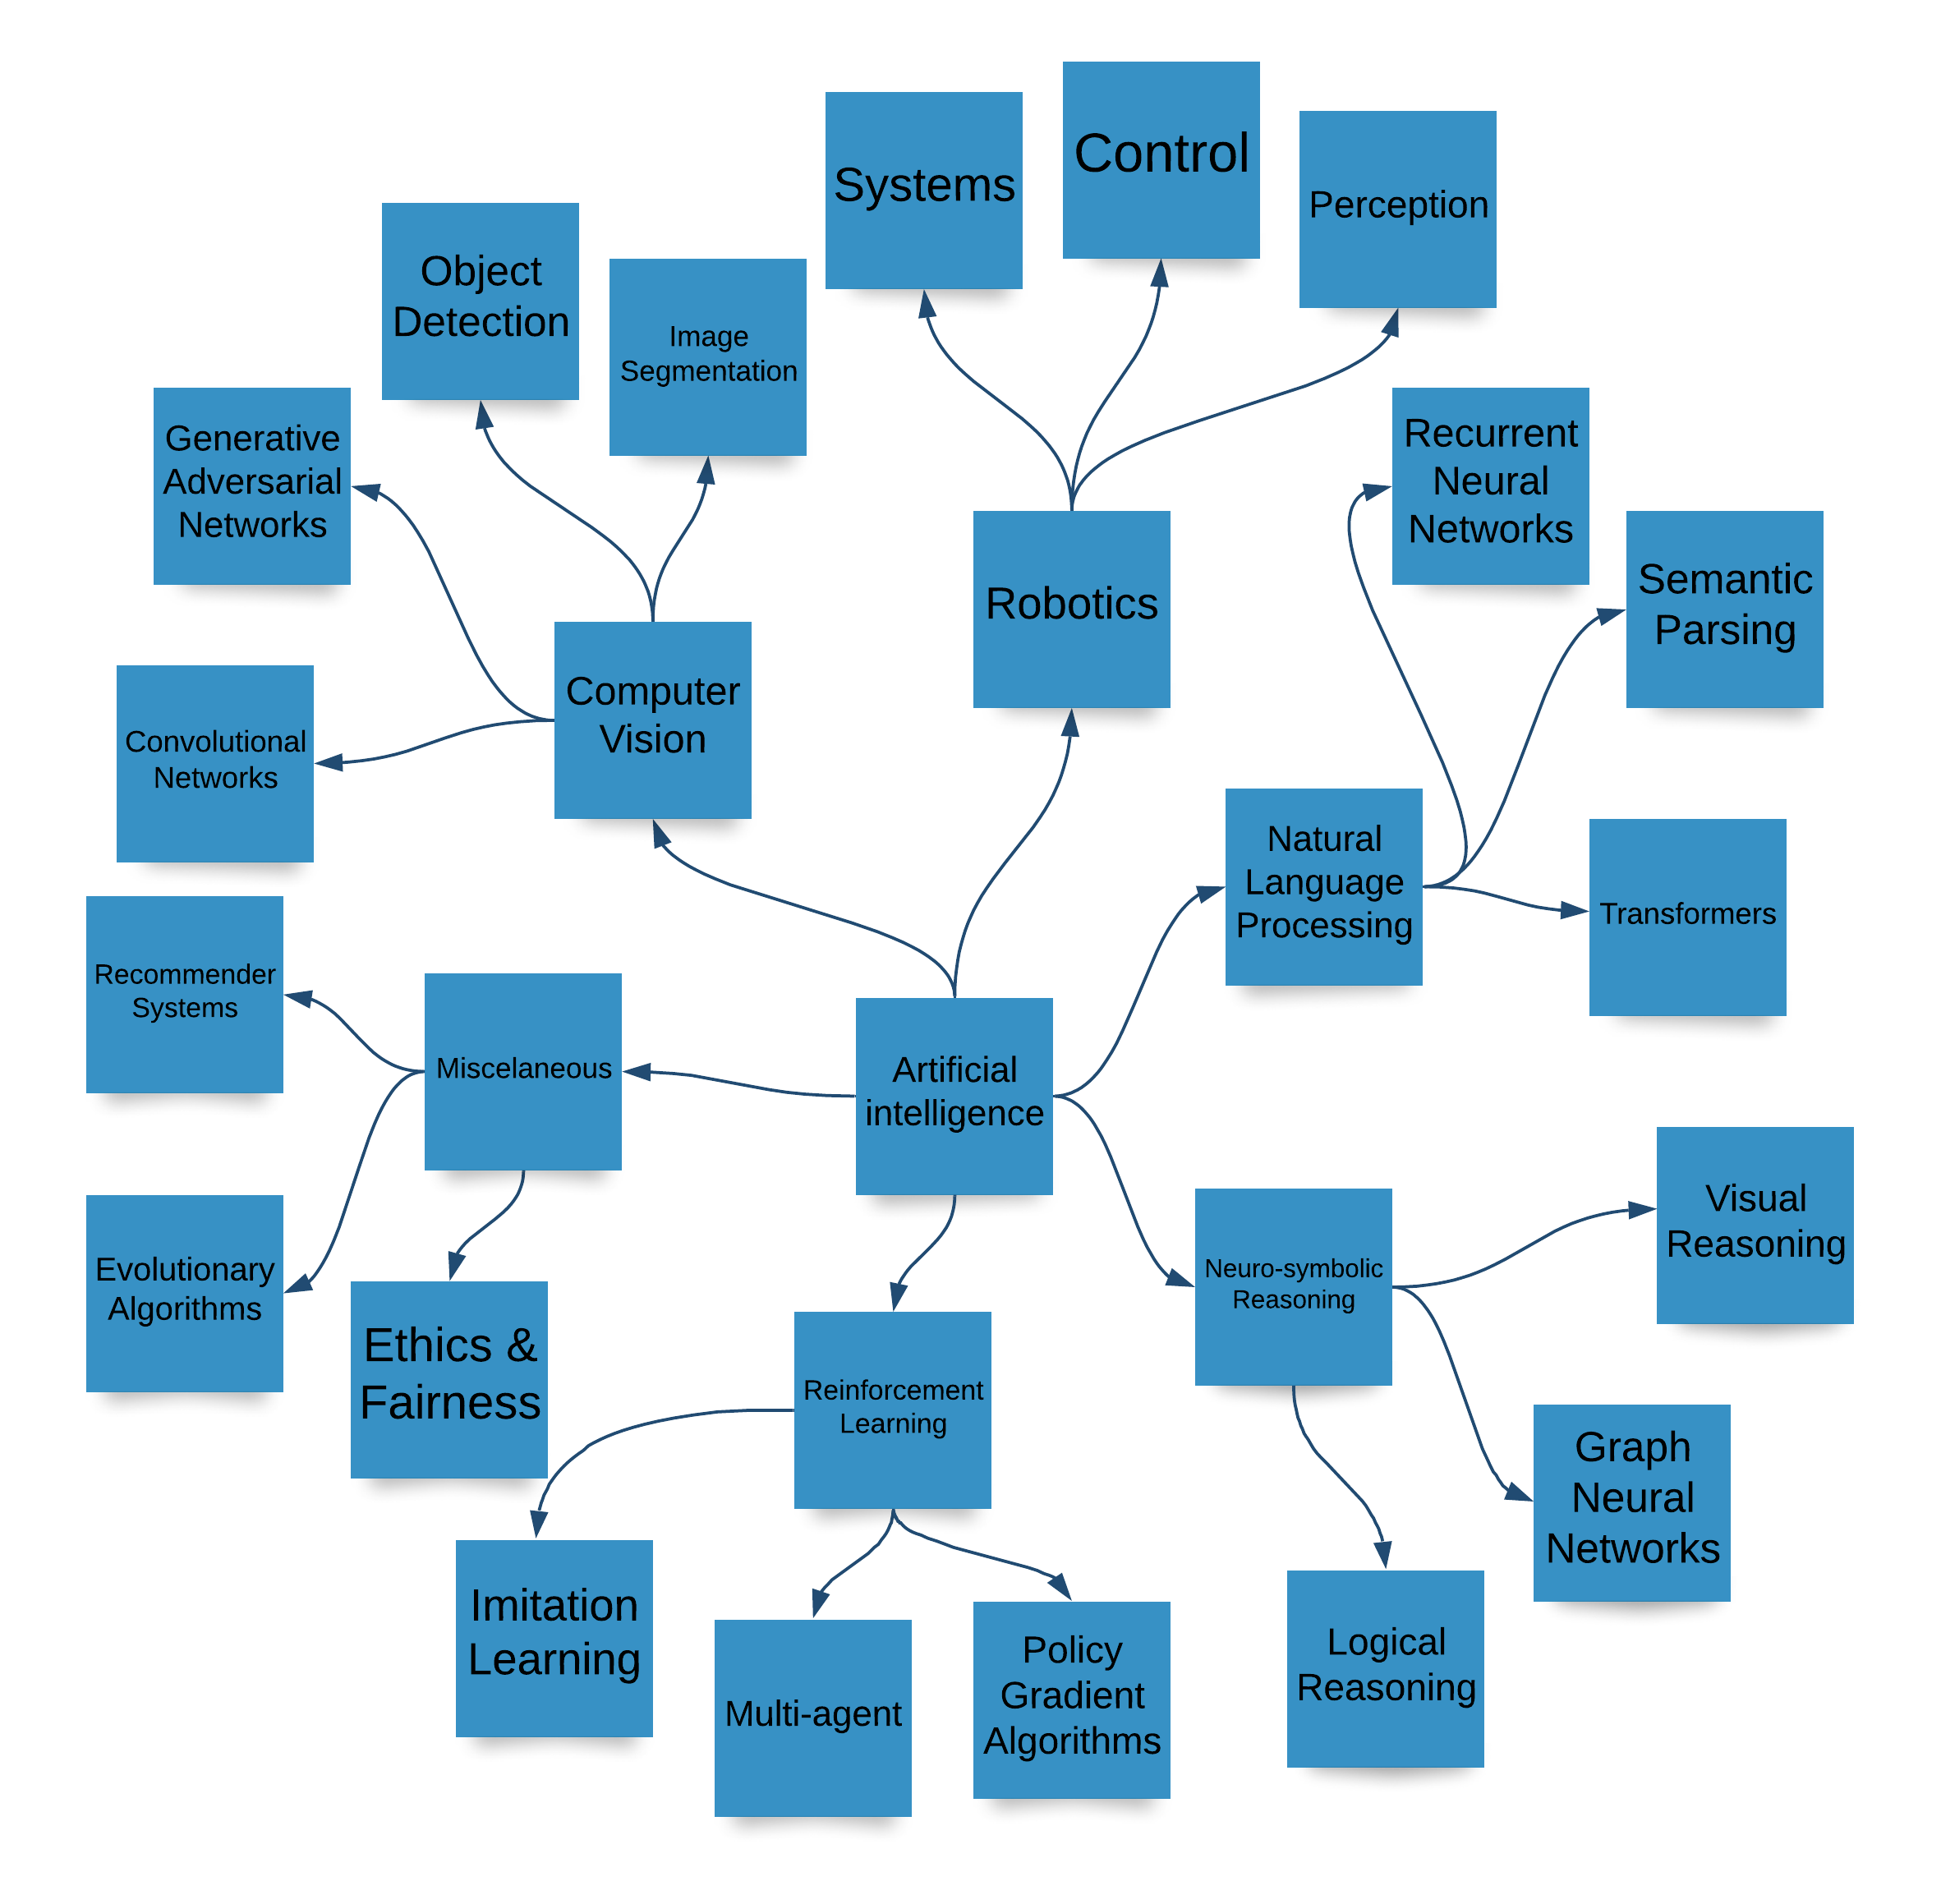
\includegraphics[width=0.85\textwidth]{figures/stoai.png}
\end{figure}

\newpage
\subsection{Deep Learning}

It is important to state the difference between the fields of \gls{ai} and \gls{dl}, since this thesis will focus mainly on the last one. 

\begin{wrapfigure}{l}{0.35\textwidth}
    \centering
    \caption{\label{fig:difference-ml-dl} Subfields Artificial Intelligence}
    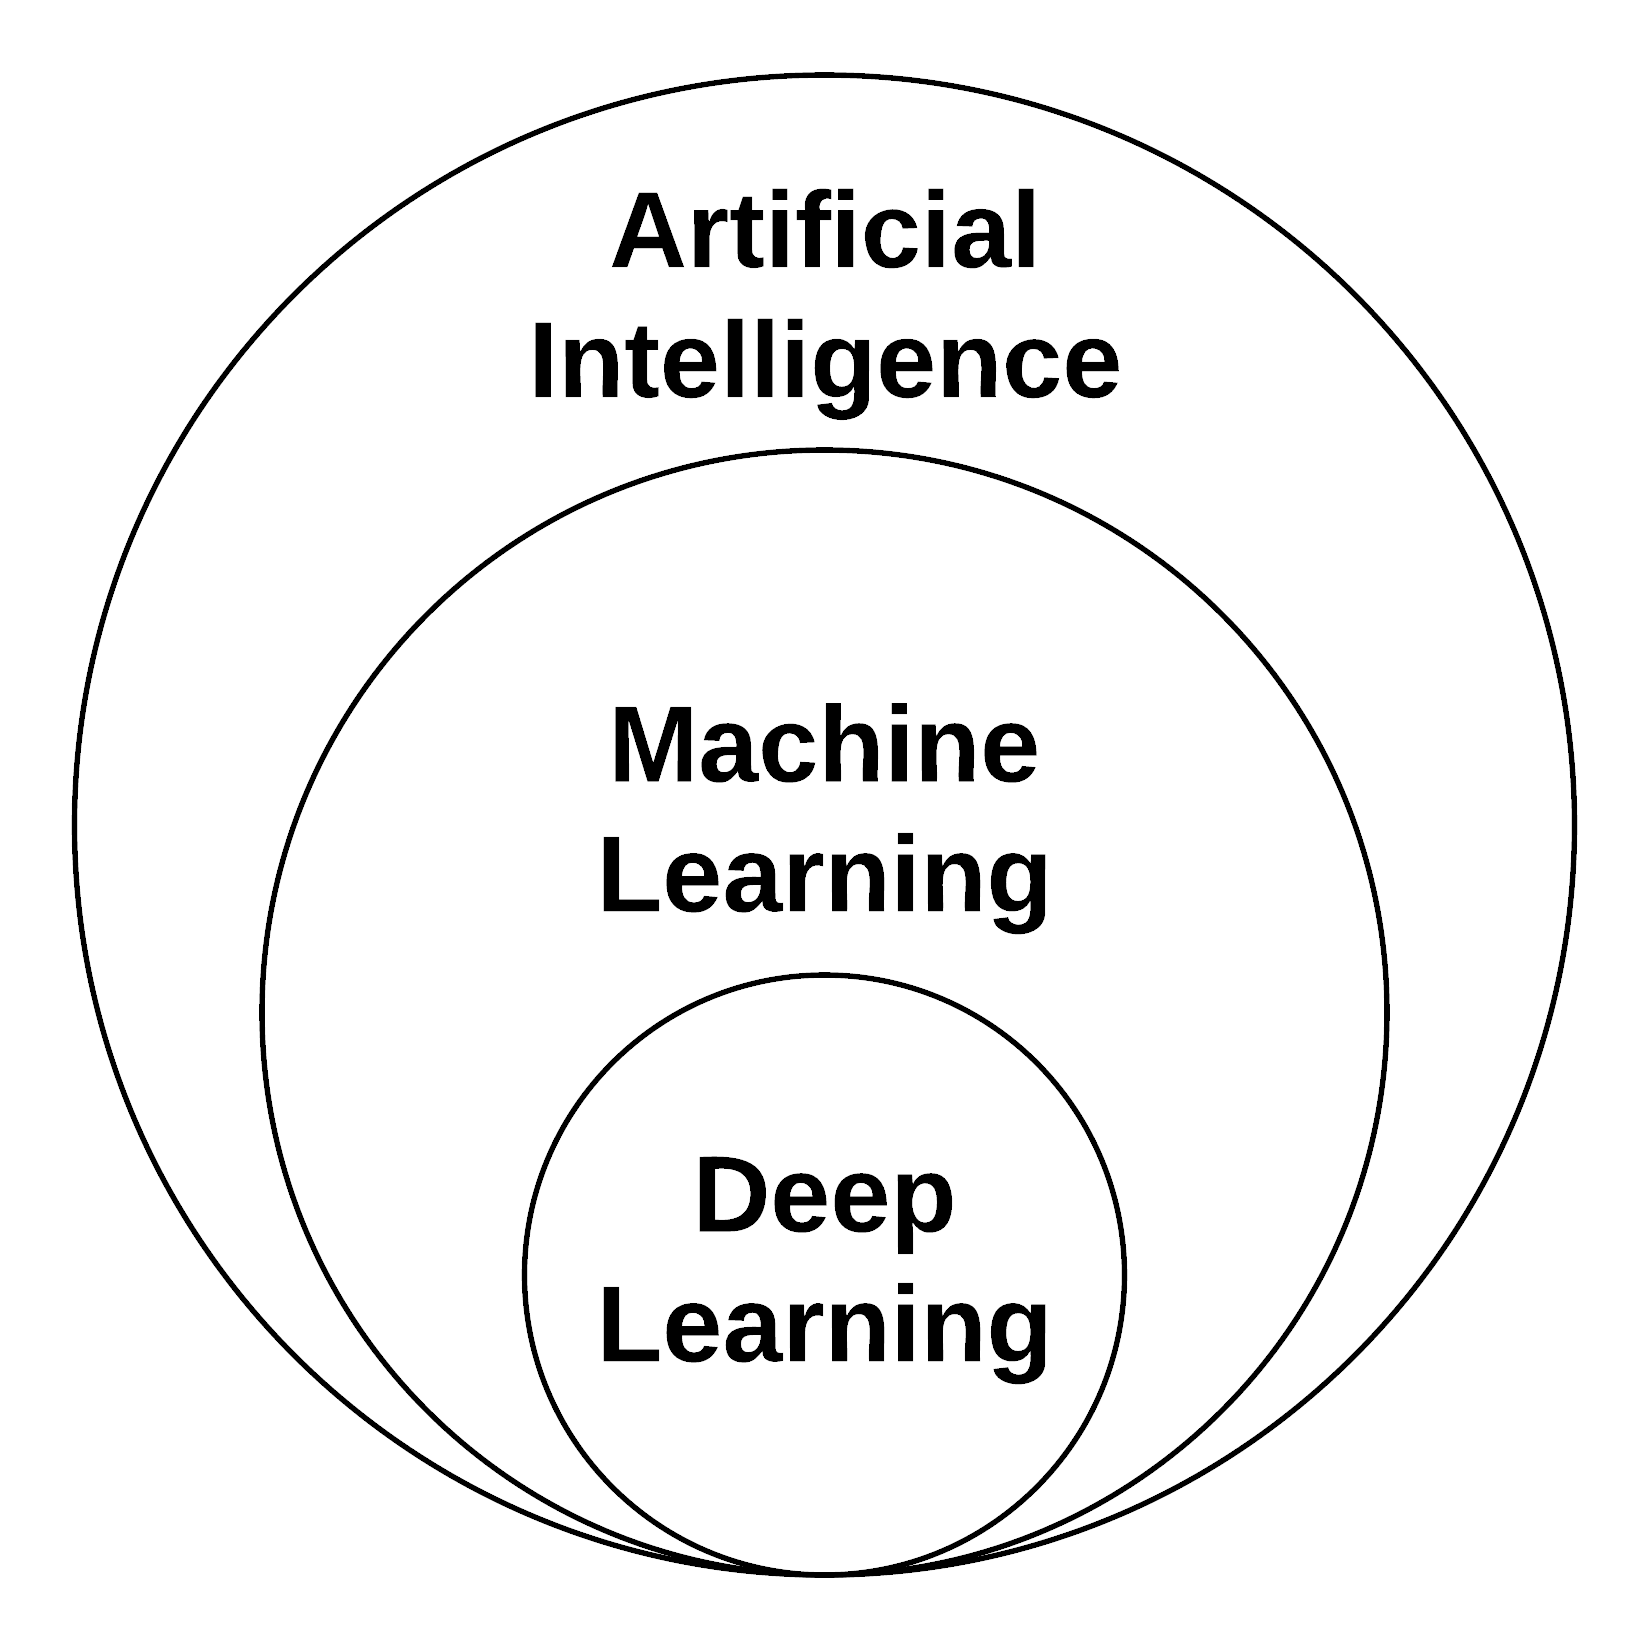
\includegraphics[width=0.3\textwidth]{figures/difference ml dl.png}
\end{wrapfigure}

\gls{dl} is a subfield of \gls{ml}, which is itself a subfield of \gls{ai}, as shown in Figure~\ref{fig:difference-ml-dl}. The main difference among each other is in the way algorithms learn. \gls{dl} algorithms automate most of the feature extraction from the data, whereas \gls{ml} relies more heavily on the experience of the person in charge of the feature engineering process.

The first \gls{nn} models were inspired by neurons and the brain's architecture, since nature has inspired many inventions throughout the history of humankind. This first model architecture was introduced by the neurophysiologist Warren McCulloch and the mathematician Walter Pitts~\cite{nnModelDefinition}.\newline

\subsection{Recurrent Neural Networks}

A \gls{rnn} looks very much like a feedforward \gls{nn}, except it also has connections pointing backward, fig~\ref{fig:memory-cell}. Since the output of a recurrent neuron at time step t is a function of all the inputs from previous time steps, you could say it has a form of memory\cite{handsOnMachine}. This feature is extremely helpful when working with time related data such as stock prices.

\begin{figure}[H]
    \centering
    \caption{\label{fig:memory-cell} Memory cell}
    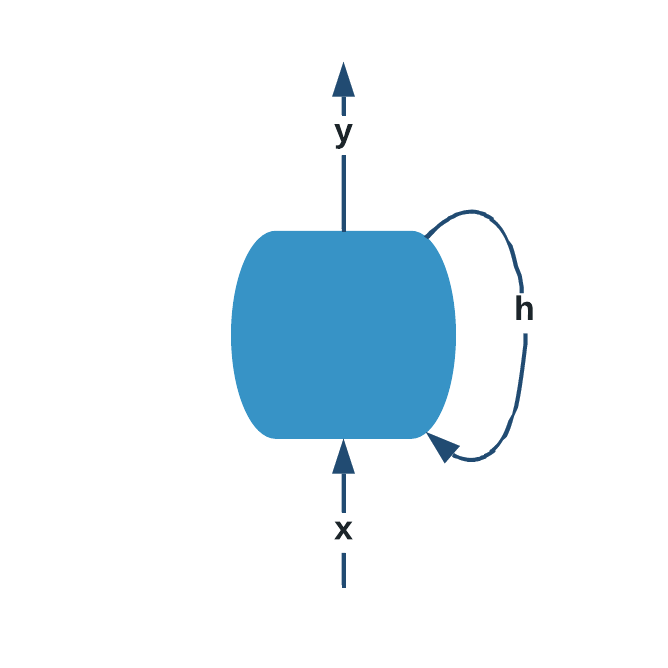
\includegraphics[width=0.30\textwidth]{figures/memory-cell.png}
\end{figure}

Due to the transformations that data undergo as it flows through an \gls{rnn}, some information is lost as time passes. After a while, the state contains practically no trace of the first entries. This phenomenon is called the vanishing gradient problem. The \gls{lstm} cell was proposed in 1997~\cite{lstm1997} by Sepp Hochreiter and Jürgen Schmidhuber and was explicitly designed to avoid the long-term dependency problem. Remembering information for long periods of time~\cite{understandLSTM}.

Although there are other approaches to deal with temporal data such as \glspl{cnn}, in this paper we will focus specifically on \gls{lstm} cells.

\section{Trading}

A trade could be defined as "the transfer of goods from one person or entity to another, often in exchange for money"~\cite{tradeDefinition}. This leads us to the natural concept of trading as an activity from which profits are expected when systematically applied. This behavior has been repeated throughout human history, as some studies show evidence of the exchange of obsidian and flint during the Stone Age~\cite{oxfordArcheology,obsidianTrade}. This phenomena can be seen as a starting point for modern economy.

Nonetheless, before further stepping into the concept of trading a clarification between the terms investing and trading is needed.

\subsection{Investing vs Trading}

Both terms are used interchangeably in a misleading manner, as they are two similar methods of attempting to make a profit~\cite{investingVsTrading}.

Investing takes a long-term approach where the goal is to gradually build wealth over a certain extended time frame by simply holding an asset the investor believes will appreciate over time, i.e., stocks, bonds, options, \glspl{etf} or real state, among others.

On the other hand, trading takes a completely different approach where the goal is to generate returns over short periods of time that outperforms holding investments by buying low and selling high. However, buying high and selling low is also a form of trading and is known as \gls{st}. There are four types of strategies depending on the period of time the trade is open for, as shown in Table~\ref{tab:types-trading}.

\begin{table}[h]
\caption{\label{tab:types-trading} Types of Trading}
\centering
\begin{tabular}{@{}|l|l|@{}}
    \toprule
    \multicolumn{1}{|c|}{\textbf{Trading Style}} & \multicolumn{1}{c|}{\textbf{Period of trade}} \\ \midrule
        Scalping         & Seconds/Minutes             \\
        Day Trading      & 1 Day                       \\
        Swing Trading    & Several days or even weeks  \\
        Position Trading & Weeks, months or even years \\ \bottomrule
\end{tabular}
\end{table}

\subsection{Machine learning applied to stock prediction}

Stock market forecasting is a fairly common topic in scientific and academic research, due to market's nature, and as mentioned previously, \gls{ml} algorithms are attracting a lot of attention in this matter due to the fact that \gls{ai} does pretty well dealing with pattern recognition. In addition to market patterns, many other macro factors can have an impact on the markets development, e.g, military conflicts, economic policies and even \textit{tweets}. All of which can be used by \gls{ai} algorithms to increase the accuracy in their predictions or decision making.

Both \gls{sl} and \gls{usl} algorithms have been used in stock market forecasting, but before steeping further into details we need a problem formulation for stock trading. "Considering the stochastic and interactive nature of the trading market, we can model it as a \gls{mdp}, which is specified as follows:"~\cite{practicalDeepLearningStock}

\begin{itemize}
    \item State \(s = [p, h, b] \): a set that includes the information of the prices of stocks p, the amount of holdings of stocks h and the remaining balance b.
    \item Action \(a\): a set of actions on all stocks. The available actions of each stock include selling, buying, and holding, which result in decreasing, increasing, and no change of the holdings h, respectively.
    \item Reward \(r(s, a, s')\): the change of the portfolio value when action a is taken at state \(s\) and arriving at the new state \(s'\).
    \item Policy \(\pi(s)\): the trading strategy of stocks at state \(s\). It is essentially the probability distribution of \(a\) at state \(s\).
    \item Action-value function \(Q\pi(s, a)\): the expected reward achieved by action \(a\) at state \(s\) following policy \(\pi\).
\end{itemize}

In their paper "Practical Deep Reinforcement Learning Approach for Stock Trading", Z. Xiong, X.-Y. Liu, S. Zhong, H. Yang y A. Walid\cite{practicalDeepLearningStock} use a \gls{ddpg} algorithm which is an improved version of the \gls{dpg} algorithm. As shown in Fig~\ref{fig:ddpg}, DDPG maintains an actor network and a critic network. The actor network \(\mu(s|\theta\mu\)) maps states to actions where \(\theta\mu\) is the set of actor network parameters, and the critic network \(Q(s, a|\theta Q)\) outputs the value of action under that state, where \(\theta Q\) is the set of critic network parameters. To explore better actions, a noise is added to the output of the actor network, which is sampled from a random process \(N\).~\cite{practicalDeepLearningStock} 

\begin{figure}[H]
    \centering
    \caption{\label{fig:ddpg} Learning Network Architecture~\cite{practicalDeepLearningStock}}
    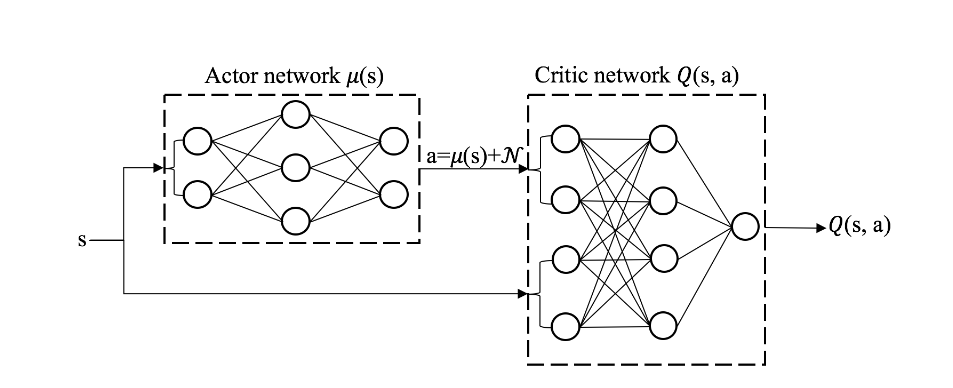
\includegraphics[width=0.85\textwidth]{figures/DDPG.png}
\end{figure}

\section{Containerization}

Over the last few years, there has been a paradigm shift in the computing field as on-premise hosted applications have gradually migrated to cloud based solutions. The concept of virtualization has played a key role in making this change possible given that some of the main advantages of cloud computing, i.e, resource efficiency, cost reduction and portability, are in part a result of virtualization technologies.

In this thesis we will talk about some different points of view of the containerization literature review. But before steeping further in, a clarifications between \gls{vm} and Container is needed.

\newpage
\subsection{Virtual Machine Vs Container}

\glspl{vm} and containers build on the same technologies and concepts. The main difference is that a \gls{vm} runs an entire \gls{os} instance on top of the "host" machine, whereas containers are intended for the deployment of single applications or services~\cite{containersStateOfArt}, as shown in Fig~\ref{fig:vm-container}

\begin{figure}[H]
    \centering
    \caption{\label{fig:vm-container} Source: www.netapp.com~\cite{vmVsContainer}}
    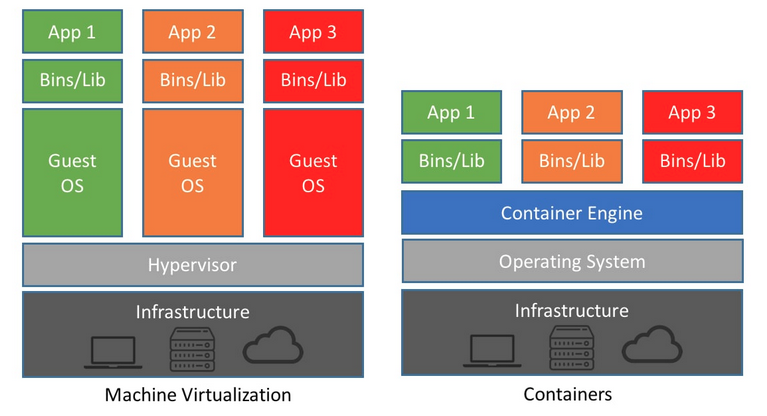
\includegraphics[width=0.65\textwidth]{figures/vm & container.png}
\end{figure}

\subsection{Orchestration}

In the container life cycle, orchestration supports automation and adaptation at run time. There are many challenges in this regard: design new processes and tools for performance monitoring, design resource and energy efficient auto scaling and scheduling algorithms and solutions for high availability. We will focus on auto scaling.

Among the auto scaling solutions, the most promising ones mix vertical and horizontal scaling and/or migration. Usually the auto scaling algorithms were designed for locally-distributed adaptation, but solutions that consider the geo-distributed case, suitable for IoT applications, have been
proposed as well. In high availability, the most promising approach is to make the detection of faulty nodes more sophisticated, e.g., based on abnormal behavior rather than only on network level or application level probes.~\cite{containersStateOfArt}

\subsection{Applications}

Containers offer an easy way to deploy Big data analytics applications based on the map-reduce or stream processing paradigms. Moreover, solutions are emerging to support the execution of containers on \gls{gpu} and \gls{fpga}, and to speedup specific analytic tasks.

Since containers are portable and have a small performance footprint, they are suitable to deploy applications on heterogeneous, resource and power limited computational units. Deploying containers on edge or fog computing nodes, or deploying containers on IoT boards like Rasperry
PI, is extremely advantageous, although it rises challenges in migration, service and resource provisioning and security.~\cite{containersStateOfArt}

\notebox{
    \textbf{"The SoTA in container technologies: Application, orchestration and security"}
    
    E. Casalicchio and S. Iannucci, provide a deep insight into different topics of containerization literature review. I strongly recommend reading their paper for those seeking a better understanding of the matter.
}

\section{Micro-services Architecture}
\label{Micro-services Architecture}

The only abstraction traditional programming languages such as C, Python or Java provide in terms of distribution and reduction of the complexity of programs is the breakdown of code into modules/packages. All of them produce single executable artifacts, also called monolith applications. Monolith applications are software programs whose modules can not be executed independently as Fig~\ref{fig:mono-app} shows. This feature generates several issues, among which:

\begin{itemize}
    \item Applications are difficult to maintain due to their larger complexity.
    \item Applications suffer from dependencies problems.
    \item Deployment processes are more complex.
    \item Scalability problems.
\end{itemize}

\begin{figure}[H]
    \centering
    \caption{\label{fig:mono-app} Source: www.n-ix.com~\cite{monoVsMicro}}
    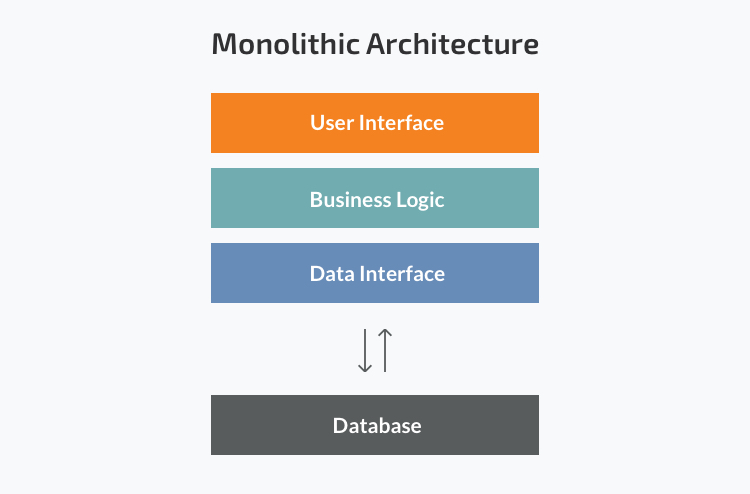
\includegraphics[width=0.5\textwidth]{figures/mono.jpg}
\end{figure}

\newpage
The micro-services architecture emerged as solution for these problems. It is in essence just a pattern that allows to decompose an application into smaller cohesive logical pieces called micro-services, mitigating most of the problems previously proposed Fig~\ref{fig:micro} . This smaller pieces communicate among each other through light messaging. Fig~\ref{fig:mono-vs-micro}

\begin{figure}[H]
    \centering
    \begin{subfigure}[a]{0.45\textwidth}
        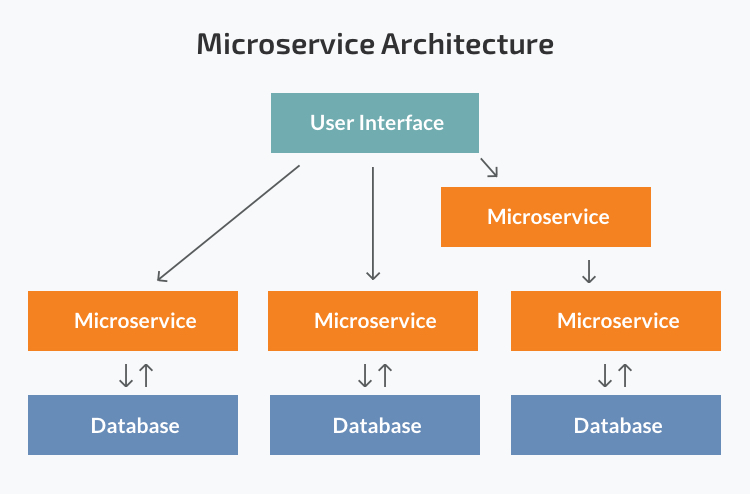
\includegraphics[width=\textwidth]{figures/micro.jpg}
        \caption{Micro-service architecture}
        \label{fig:micro}
    \end{subfigure}
    \hfill
    \begin{subfigure}[b]{0.54\textwidth}
        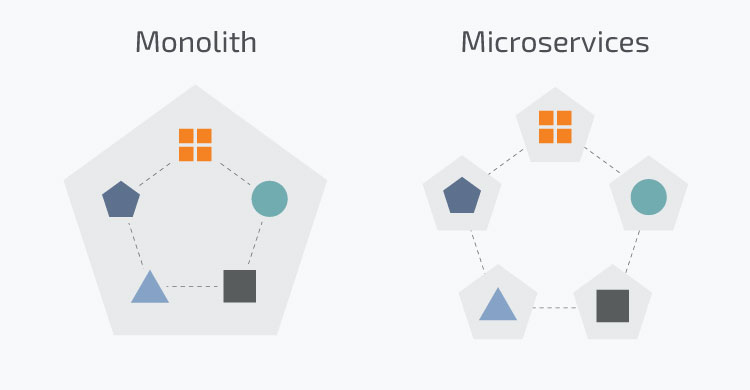
\includegraphics[width=\textwidth]{figures/micro vs mono.jpg}
        \caption{Monolith vs Micro-services}
        \label{fig:mono-vs-micro}
    \end{subfigure}
    \caption{\label{fig:mono-micro}www.n-ix.com~\cite{monoVsMicro}}
\end{figure}

\subsection{Today}

"Micro-services now are a new trend in software architecture, which emphasises the design and development of highly maintainable and scalable software. Micro-services manage growing complexity by functionally decomposing large systems into a set of independent services. By making services completely independent in development and deployment, microservices emphasise loose coupling and high cohesion by taking modularity to the next level. This approach delivers all sorts of benefits in terms of maintainability, scalability, and so on.[...].The micro-service architecture still shows distinctive characteristics that blend into something unique and different from \gls{soa} itself.[..]. The micro-service architecture gained popularity relatively recently and can be considered to be in its infancy since there is still a lack of consensus on what micro-services actually are."~\cite{microservicesStateOfArt} Hence, micro-services offer a new modularity in software architecture that had not been practiced before and thus it has created a paradigm shift in this field of computation.

\subsection{Tomorrow}

"The greatest strength of micro-services comes from pervasive distribution: even the internal components of software are autonomous services, leading to loosely coupled systems and the other benefits previously discussed. However, from this same aspect (distribution) also comes its greatest weakness: programming distributed systems is inherently harder than monoliths. We now have to think about new issues. Some examples are how can we manage changes to a service that may have side effects on other services that it communicates with? How can we prevent attacks that exploit network communications?.[...] There are many pitfalls that we need to keep in mind when programming with
micro services:"~\cite{microservicesStateOfArt} a) Interfaces; b) Behavioural specifications and choreographies; c) Greater surface attack area; d) Network complexity; e) Trust.

\begin{itemize}
    \item Interfaces.
    \item Behavioural Specifications and Choreographies.
    \item Greater Surface Attack Area.
    \item Network Complexity.
    \item Trust.
\end{itemize}

\chapter{Methodology}
\label{mt:methodology}

In this section, we will walk through all the organizational aspects related to the project: configuration management, \gls{ci}/\gls{cd} workflows, micro-service architecture structure and model definition.

\section{Configuration Management}

Configuration management can be defined as a process that ensures the consistency and quality of a project/product through its life cycle and the various changes it undergoes. Sometimes the term is mistaken for version control, but in fact configuration management includes version control.

In this subsection we will talk about the different technologies and tools that have been used in order to keep a decent control of configuration management.

\subsection{Git \& GitHub}

As mentioned above, version control is a part of configuration management and is responsible for recognizing and managing the various changes of software code. Version control systems are software tools that help teams manage changes to source code over time. 

For this project Git has been the clear option since it is the market leader due to its huge speed and its branch and merge functionality, among others. Taken from its website \enquote{Git is a free and open source distributed version control system designed to handle everything from small to very large projects with speed and efficiency}.~\cite{gitDefinition}

GitHub is essentially a remote repository hosting platform for Git. It allows developers to work together on the same project from anywhere. Figure~\ref{fig:current-status-github} presents an example.

\begin{figure}[H]
    \centering
    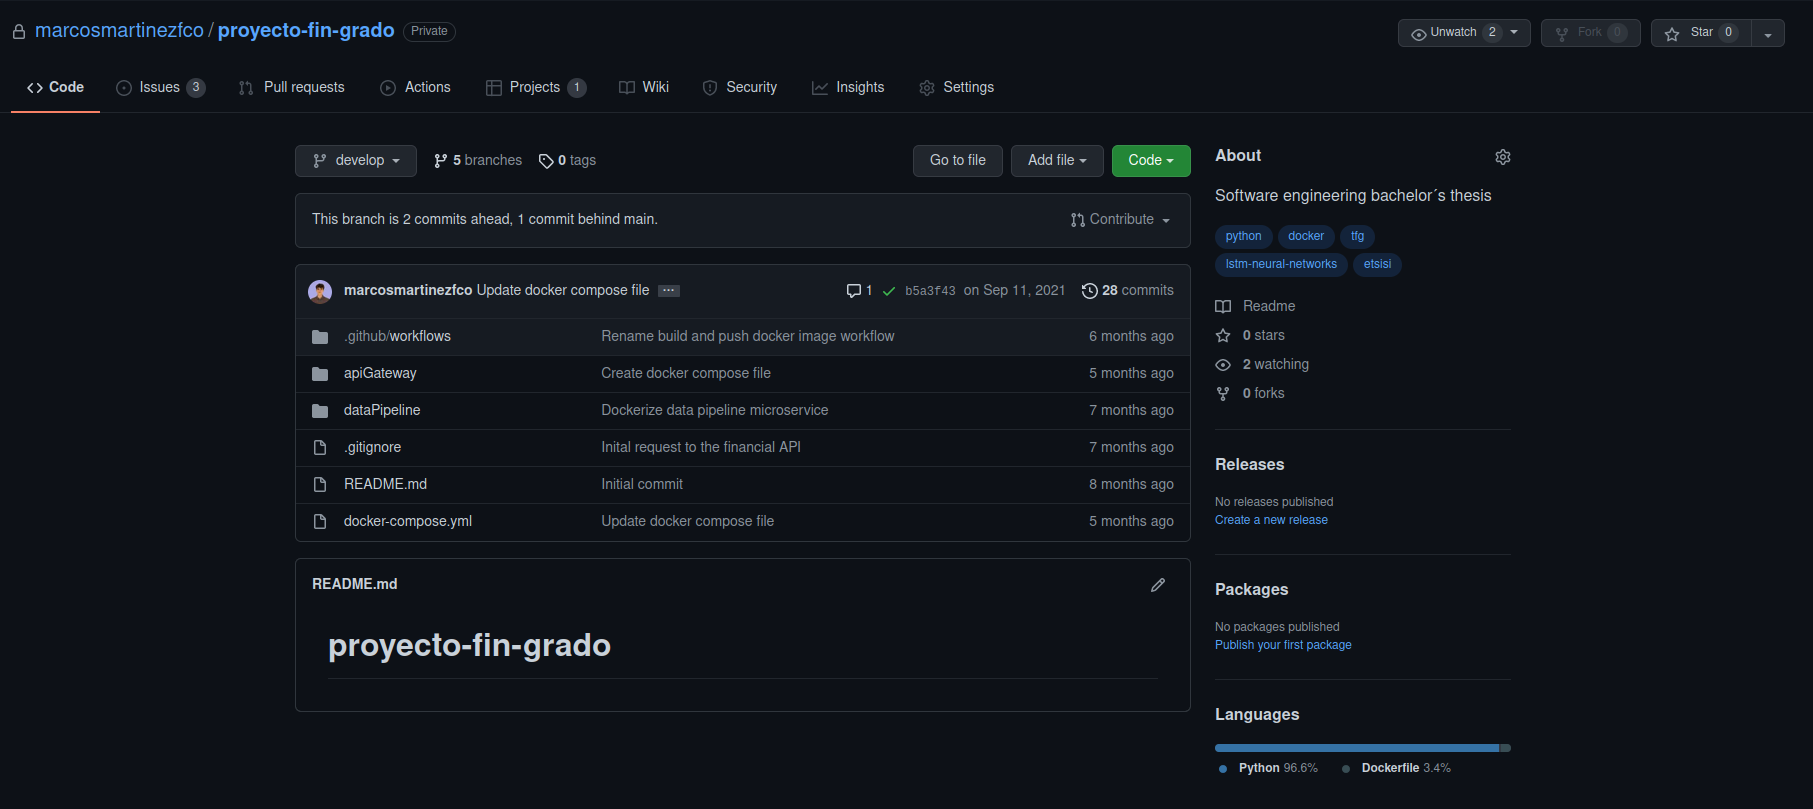
\includegraphics[width=\textwidth]{figures/github.png}
    \caption{GitHub Repository}
    \label{fig:current-status-github}
\end{figure}

\subsection{Git Workflow}

A Git workflow is a template for how to use git to accomplish work in a consistent and productive manner. Git is extremely flexible when it comes to managing changes, so there is no imposed or standardized process. When working with a team on a project, it is important to make sure that the entire team is familiar with how changes will be applied. 

Gitflow has been chosen for this project because of its versatility and the ability to generate branches for each of the features needed for the project, Figure~\ref{fig:gitflow-example}. In our case, it will be extremely useful to be able to develop each of the modules/micro-services of the system in parallel.

\begin{figure}[H]
    \centering
    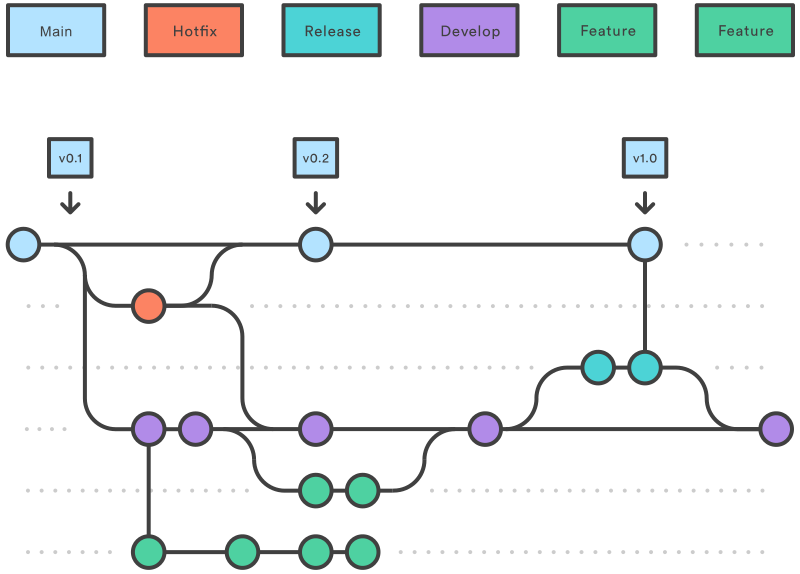
\includegraphics[width=0.55\textwidth]{figures/gitflow.png}
    \caption{Gitflow Scheme, Source: www.atlassian.com~\cite{gitflow}}
    \label{fig:gitflow-example}
\end{figure}

\subsection{GitHub Projects}

When planning a project, one of the most important tasks is the identification and organization of the necessary work to do in order to complete the project. Due to the changing nature of a degree's thesis and all its uncertainties, agile methodologies seem to be the clear choice to organize its planning and be able to adapt to any change or problem that may appear during its different stages. For this specific thesis different agile methodologies have been used to enhance its development, among which sprints~\footnote{Short, time-boxed period when a scrum team works to complete a set amount of work.~\cite{sprintsDef}} and \gls{Kanban} boards~\footnote{Agile project management tool designed to help visualize work, limit work-in-progress, and maximize efficiency.~\cite{kanbanDef}} stand out.

GitHub provides a helpful tool for creating and managing \gls{Kanban} boards called projects. Figure~\ref{fig:github-projects} shows a snapshot of my project backlog. Task can be either added, edited or deleted from the backlog. They can also be transferred among stages and you can even link them to pull requests or issues which is extremely convenient for workflow automation, since tasks can be automatically transferred around depending on the outcome of those issues/pull requests.

As for the sprints, every two weeks I would meet with my mentor to review the status of the project and discuss about the next steps to take. After that, all the decisions were reflected on the backlog hosted in the GitHub projects, until the end of the newly started sprint.

\begin{figure}[h]
    \centering
    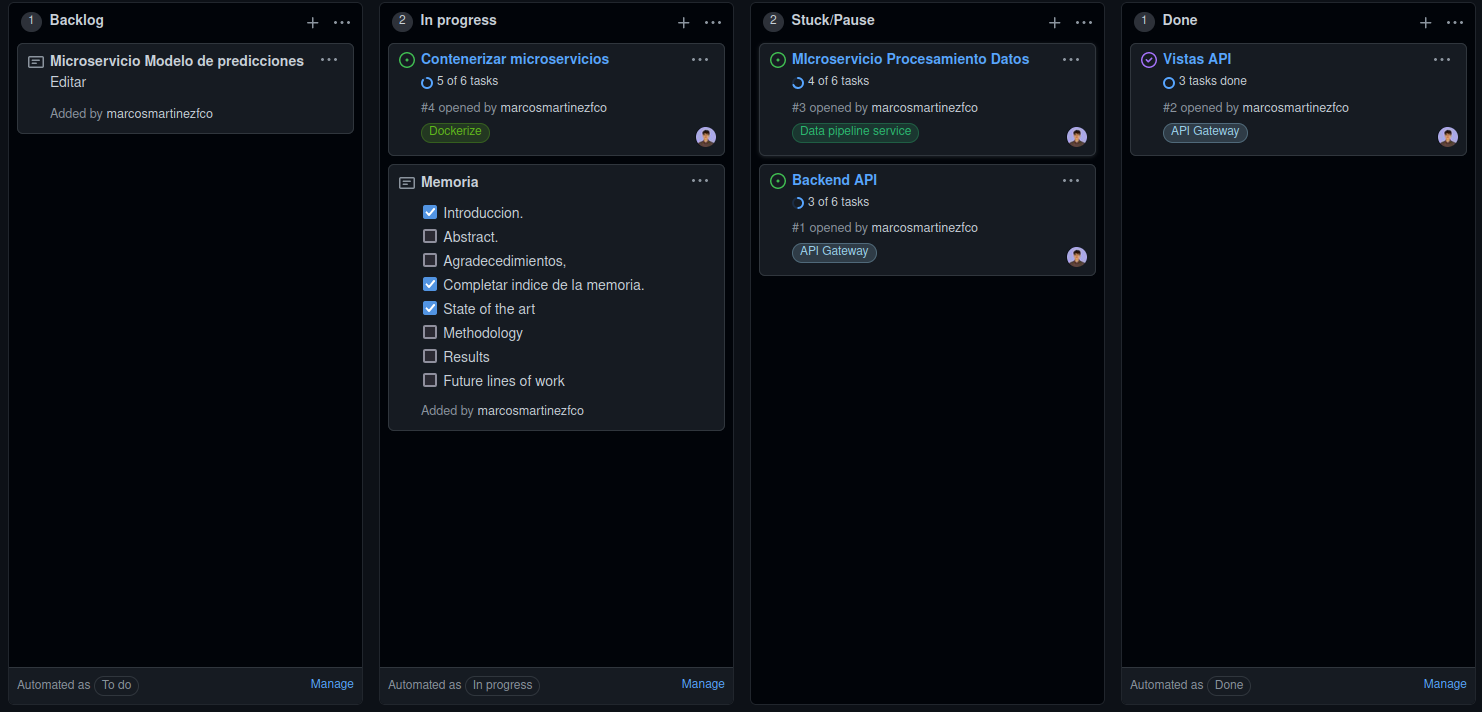
\includegraphics[width=\textwidth]{figures/github-projects.png}
    \caption{Github Projects Kanban}
    \label{fig:github-projects}
\end{figure}

\section{CI/CD Workflows}

One of the main goals during the design phase of this thesis is to have a high level of automation to be able to maintain all the different development processes related to micro-services. Luckily GitHub provides us with a powerful tool for creating custom workflow pipelines, called GitHub actions. These workflows must be located in a folder called \textbf{.github/workflows}, in the root of the repository in different "YAML" files.

GitHub actions fees depend on computing time and the runner's \gls{os}. Runners are responsible for executing the different jobs specified in a workflow, Tab~\ref{tab:action-fees} shows the different prices.

\begin{table}[h]
\centering
\caption{Runner Fees}
\label{tab:action-fees}
\begin{tabular}{@{}ll@{}}
\toprule
Linux             & \$0.008/min \\ \midrule
Windows           & \$0.016/min \\ \midrule
macOs             & \$0.08/min  \\ \midrule
Self-hosted       & Free        \\ \midrule
Public repository & Free       
\end{tabular}
\end{table}

\subsection{Self-hosted Runner}

\begin{lstlisting}[language=bash, caption=Set up Self-hosted Runner,label={lst:self-hosted-runner}]
$ curl -o actions-runner-linux-x64-2.287.1.tar.gz -L https://github.com/actions/runner/releases/download/v2.287.1/actions-runner-linux-x64-2.287.1.tar.gz
$ tar xzf ./actions-runner-linux-x64-2.287.1.tar.gz
$ ./config.sh --url https://github.com/username/repository --token "YOUR TOKEN"
$ ./run.sh
$ sudo ./svc.sh install #this will create a systemd daemon to start the runner on start up
\end{lstlisting}

Self-hosted runners offer more control of hardware, \gls{os}, and software tools than GitHub-hosted runners provide. With self-hosted runners, you can choose to create a custom hardware configuration with more processing power or memory to run larger jobs, install software available on your local network, and choose an \gls{os} not offered by GitHub-hosted runners. Self-hosted runners can be physical, virtual, in a container, on-premises, or in a cloud~\cite{selfHostedRunner}.

To add a self-hosted runner, is as simple as going to the actions section in the repository settings and follow the instructions, Listing~\ref{lst:self-hosted-runner} shows the steps used to configure a Linux based runner for the project. From now on, our self-hosted runner will listen for jobs from our GitHub repository and start executing them whenever a workflow is triggered.

\subsection{Workflow Definition}

Two of the most important aspects to take into consideration when defining a workflow, are the branches or events that will trigger it and the jobs and tasks to be executed. Note that these jobs do not necessarily have to be sequentially executed, in fact they run in parallel by default. Nonetheless, GitHub actions allows us to establish dependencies between jobs, so that certain ones are executed before others.

Triggering events must be defined under the \enquote{on}: tag. Listing~\ref{lst:trigger-options} shows an example of a couple of interesting ones, for more information about triggering events follow the instructions in the action's documentation.

\begin{lstlisting}[caption=Common Workflow Triggers,label={lst:trigger-options}]
on:
  push:
    branches: [only when specific branches are pushed]
    branches-ignore: [ignored branches]
    paths: # triggers when a push to specific files occurs
        - '**.sol'
  pull_request:
    types: [pull request activity type]
  workflow_dispatch: # allows the workflow to be triggered manually
\end{lstlisting}

As for the job definition, they all must be declared under the \enquote{job} tag. Jobs run in parallel by default as we explained before. To run them sequentially, you can define dependencies as Listing~\ref{lst:jobs-definition} shows. Also, the runner which will execute the job, needs to be chosen in the definition.

\begin{lstlisting}[caption=Job Dependencies Definition,label={lst:jobs-definition}]
jobs:
  jobA:
    runs-on: [self-hosted] # the job will be forwarded to our self-hosted runner
  jobB:
    runs-on: [ubuntu-latest] # the job will be executed in a hosted ubuntu machine
    needs: jobA
  jobC:
    runs-on: [self-hosted]
    if: ${{ always() }} #jobC will execute regardless of jobA & jobB output
    needs: [jobA, jobB]
\end{lstlisting}

The most powerful feature about GitHub actions is the integration with its whole ecosystem. So for instance, each job has a list of steps which are always executed sequentially and they all need to pass, in order for the job to successfully finish. These task can be either manually specified or reused from the Action's marketplace, where everyone can either upload or reuse published actions. To use any of them, is as simple as specifying the dependency \enquote{publisher/actions@version}. Listing~\ref{lst:step-definition} shows an example of a reused action from the marketplace.

Another useful feature is the \enquote{secrets} environment, which lets you define repository level environment variables that need to be off the code, i.e, \gls{api} keys, tokens or cryptography private keys.

\begin{lstlisting}[caption=Steps Definition,label={lst:step-definition}]
steps:
- uses: actions/first-interaction@v1 # dependency definition
  with:
    repo-token: ${{ secrets.GITHUB_TOKEN }} # GitHub environment variable
    issue-message: 'message that will be displayed on users' first issue'
    pr-message: 'message that will be displayed on users' first pr'
\end{lstlisting}

\subsection{Build \& Push Workflow}

As shown in Listing~\ref{lst:build-push-docker}, \enquote{Build-push-docker-images.yml} describes the workflow used for building and pushing the different docker images used in the project into docker hub. Automating all code deployment generated during development.

\begin{lstlisting}[caption=build-push-docker-images.yml,label={lst:build-push-docker}]
name: Build an push docker images to docker hub
on:
  push:
    branches: [main , develop]
  workflow_dispatch:
jobs:
  build:
    runs-on: self-hosted
    steps:
      - name: Repo checkout
        uses: actions/checkout@v2
      - name: Docker Login
        uses: docker/login-action@v1.10.0
        with:
          username: ${{secrets.DOCKER_USERNAME}}
          password: ${{secrets.DOCKER_TOKEN}}
      - name: Build and push api-gateway image
        uses: docker/build-push-action@v2
        with:
          context: apiGateway/
          push: true
          tags: marcosmartinezfco/tfg-api-gateway:latest
      - name: Build and push data-pipeline image
        uses: docker/build-push-action@v2
        with:
          context: dataPipeline/
          push: true
          tags: marcosmartinezfco/tfg-data-pipeline:latest
\end{lstlisting}

\section{Micro-service Architecture}
\label{Micro-service Architecture}

In section~\ref{Micro-services Architecture} we introduced the micro-service architecture pattern and its features. This section will focus in the different technologies that have been used to implement the pattern and the general layout of the application.

\begin{figure}[h]
    \centering
    \caption{Architecture Layout}
    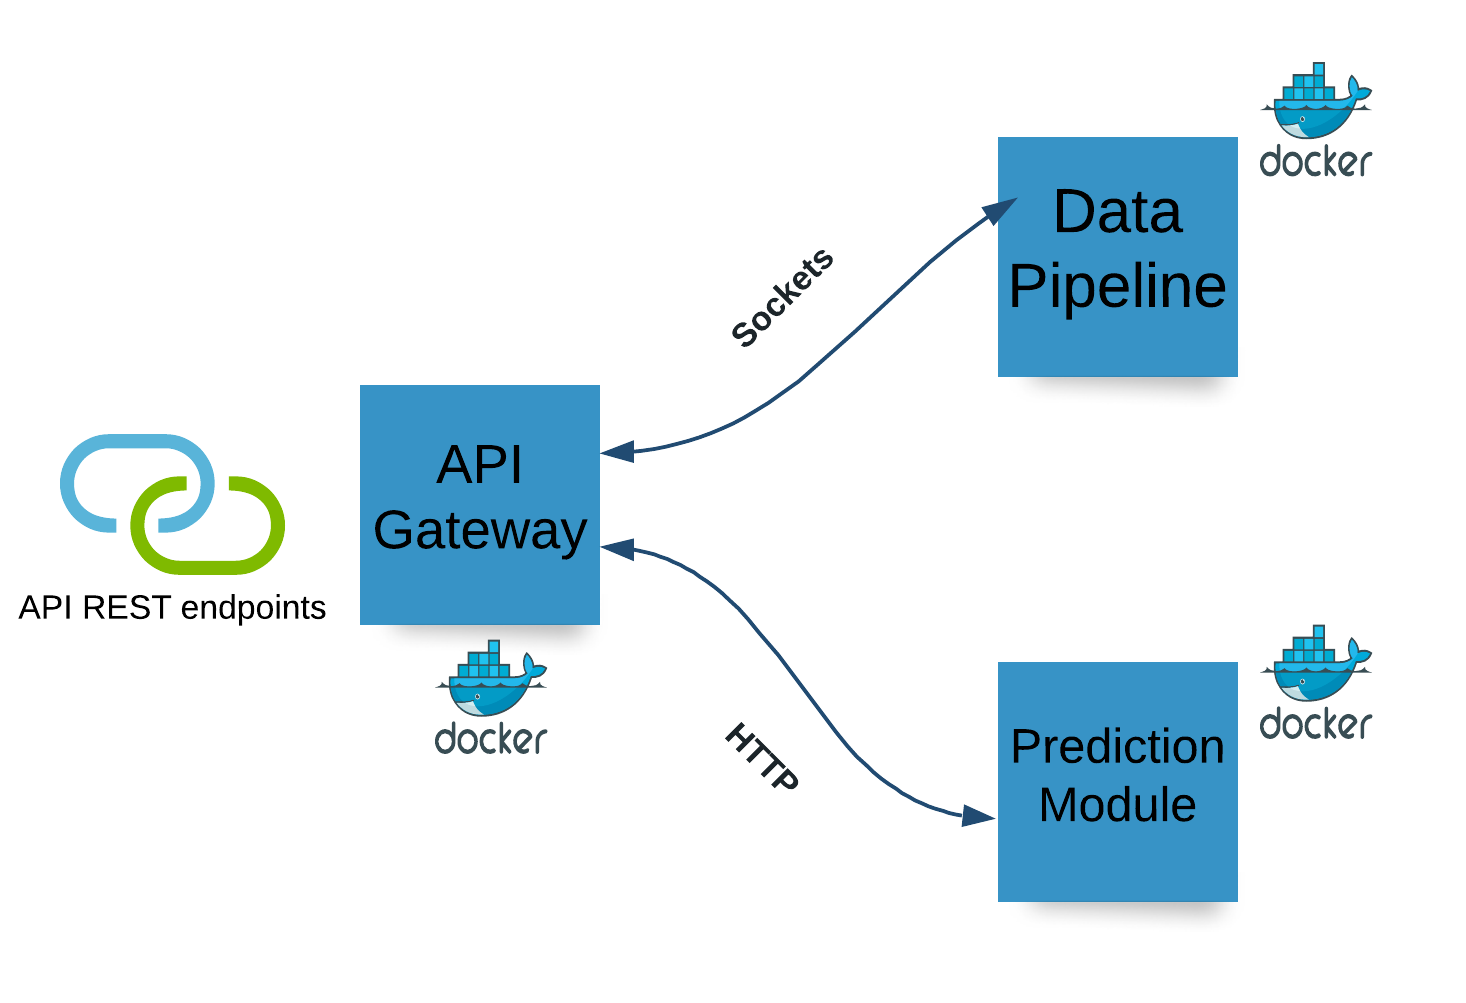
\includegraphics[width=\textwidth]{figures/architecture.png}
    \label{fig:architecture-layout}
\end{figure}

Figure~\ref{fig:architecture-layout} shows all the micro-services the architecture is decomposed into, each of which is an independent docker container as we previously have mentioned:

\begin{itemize}
    \item \gls{api} Gateway is the module that provides the endpoints users will use to get the predictions.
    \item Data pipeline is the module in charge of downloading the historical data of an asset which will be fed to the model in order to get the prediction for that asset.
    \item The prediction module is in charge of receiving a time-series with historical data of a company and then forecasting a prediction of the closing price. We will be using the battle tested tool Tensorflow Serve to implement this micro-service.
\end{itemize}

\subsection{Container communication}
\label{Container communication}

 Given the fact that containers act as an isolated system from the host and seeing Figure~\ref{fig:architecture-layout}, a natural question arise. How do these containers communicate with one another?
 
 One of the main reasons for Docker popularity is containers and services do not even need to be aware that they are deployed on Docker, or the host's \gls{os}, or whether their peers are also Docker workloads or not. You can use Docker to manage containers in a platform-agnostic way through Docker networking drivers~\cite{dockerNetworking}. These drivers allow you to specify how containers should behave and communicate, as Table~\ref{tab:docker-drivers} shows.
 
\begin{table}[h]
\centering
\caption{Docker Network Drivers}
\label{tab:docker-drivers}
\begin{tabular}{@{}|c|l|@{}}
\toprule
\textbf{Driver} & \multicolumn{1}{c|}{\textbf{Funcitonality}}                                                                                            \\ \midrule
Bridge          & \begin{tabular}[c]{@{}l@{}}Is best when you need multiple\\ containers to communicate on the same host.\end{tabular}                   \\ \midrule
Host            & \begin{tabular}[c]{@{}l@{}}Removes network isolation between \\ the container and the host, using its networking directly.\end{tabular} \\ \midrule
Overlay &
  \begin{tabular}[c]{@{}l@{}}Is best when you need containers running on \\ different hosts to communicate. It connects multiple Docker \\ daemons together, removing the need to do OS-level routing.\end{tabular} \\ \midrule
macVLAN &
  \begin{tabular}[c]{@{}l@{}}Allows you to assign a MAC address to a container,\\ making it appear as a physical device on your network.\end{tabular} \\ \midrule
Custom          & Third-party network plugins.                                                                                                           \\ \midrule
None            & It disables all networking, usually used together with a custom driver.                                                                \\ \bottomrule
\end{tabular}
\end{table}

This project uses the bridge driver since the host machine houses all the orchestration. On their own, bridge networks provide a software networking layer which allows connected containers to communicate, while providing full isolation from containers that are not connected.

Docker creates a bridge network by default to which all containers are connected if not specified otherwise. These containers can reference one another based on their IP address. User-defined networks can also be created, with the advantage of more configuration capabilities and containers being able to reference one another by their name instead of an IP address. Fig~\ref{fig:tfg-net} shows the user-defined bridge network used in this project.

\begin{figure}[h]
    \centering
    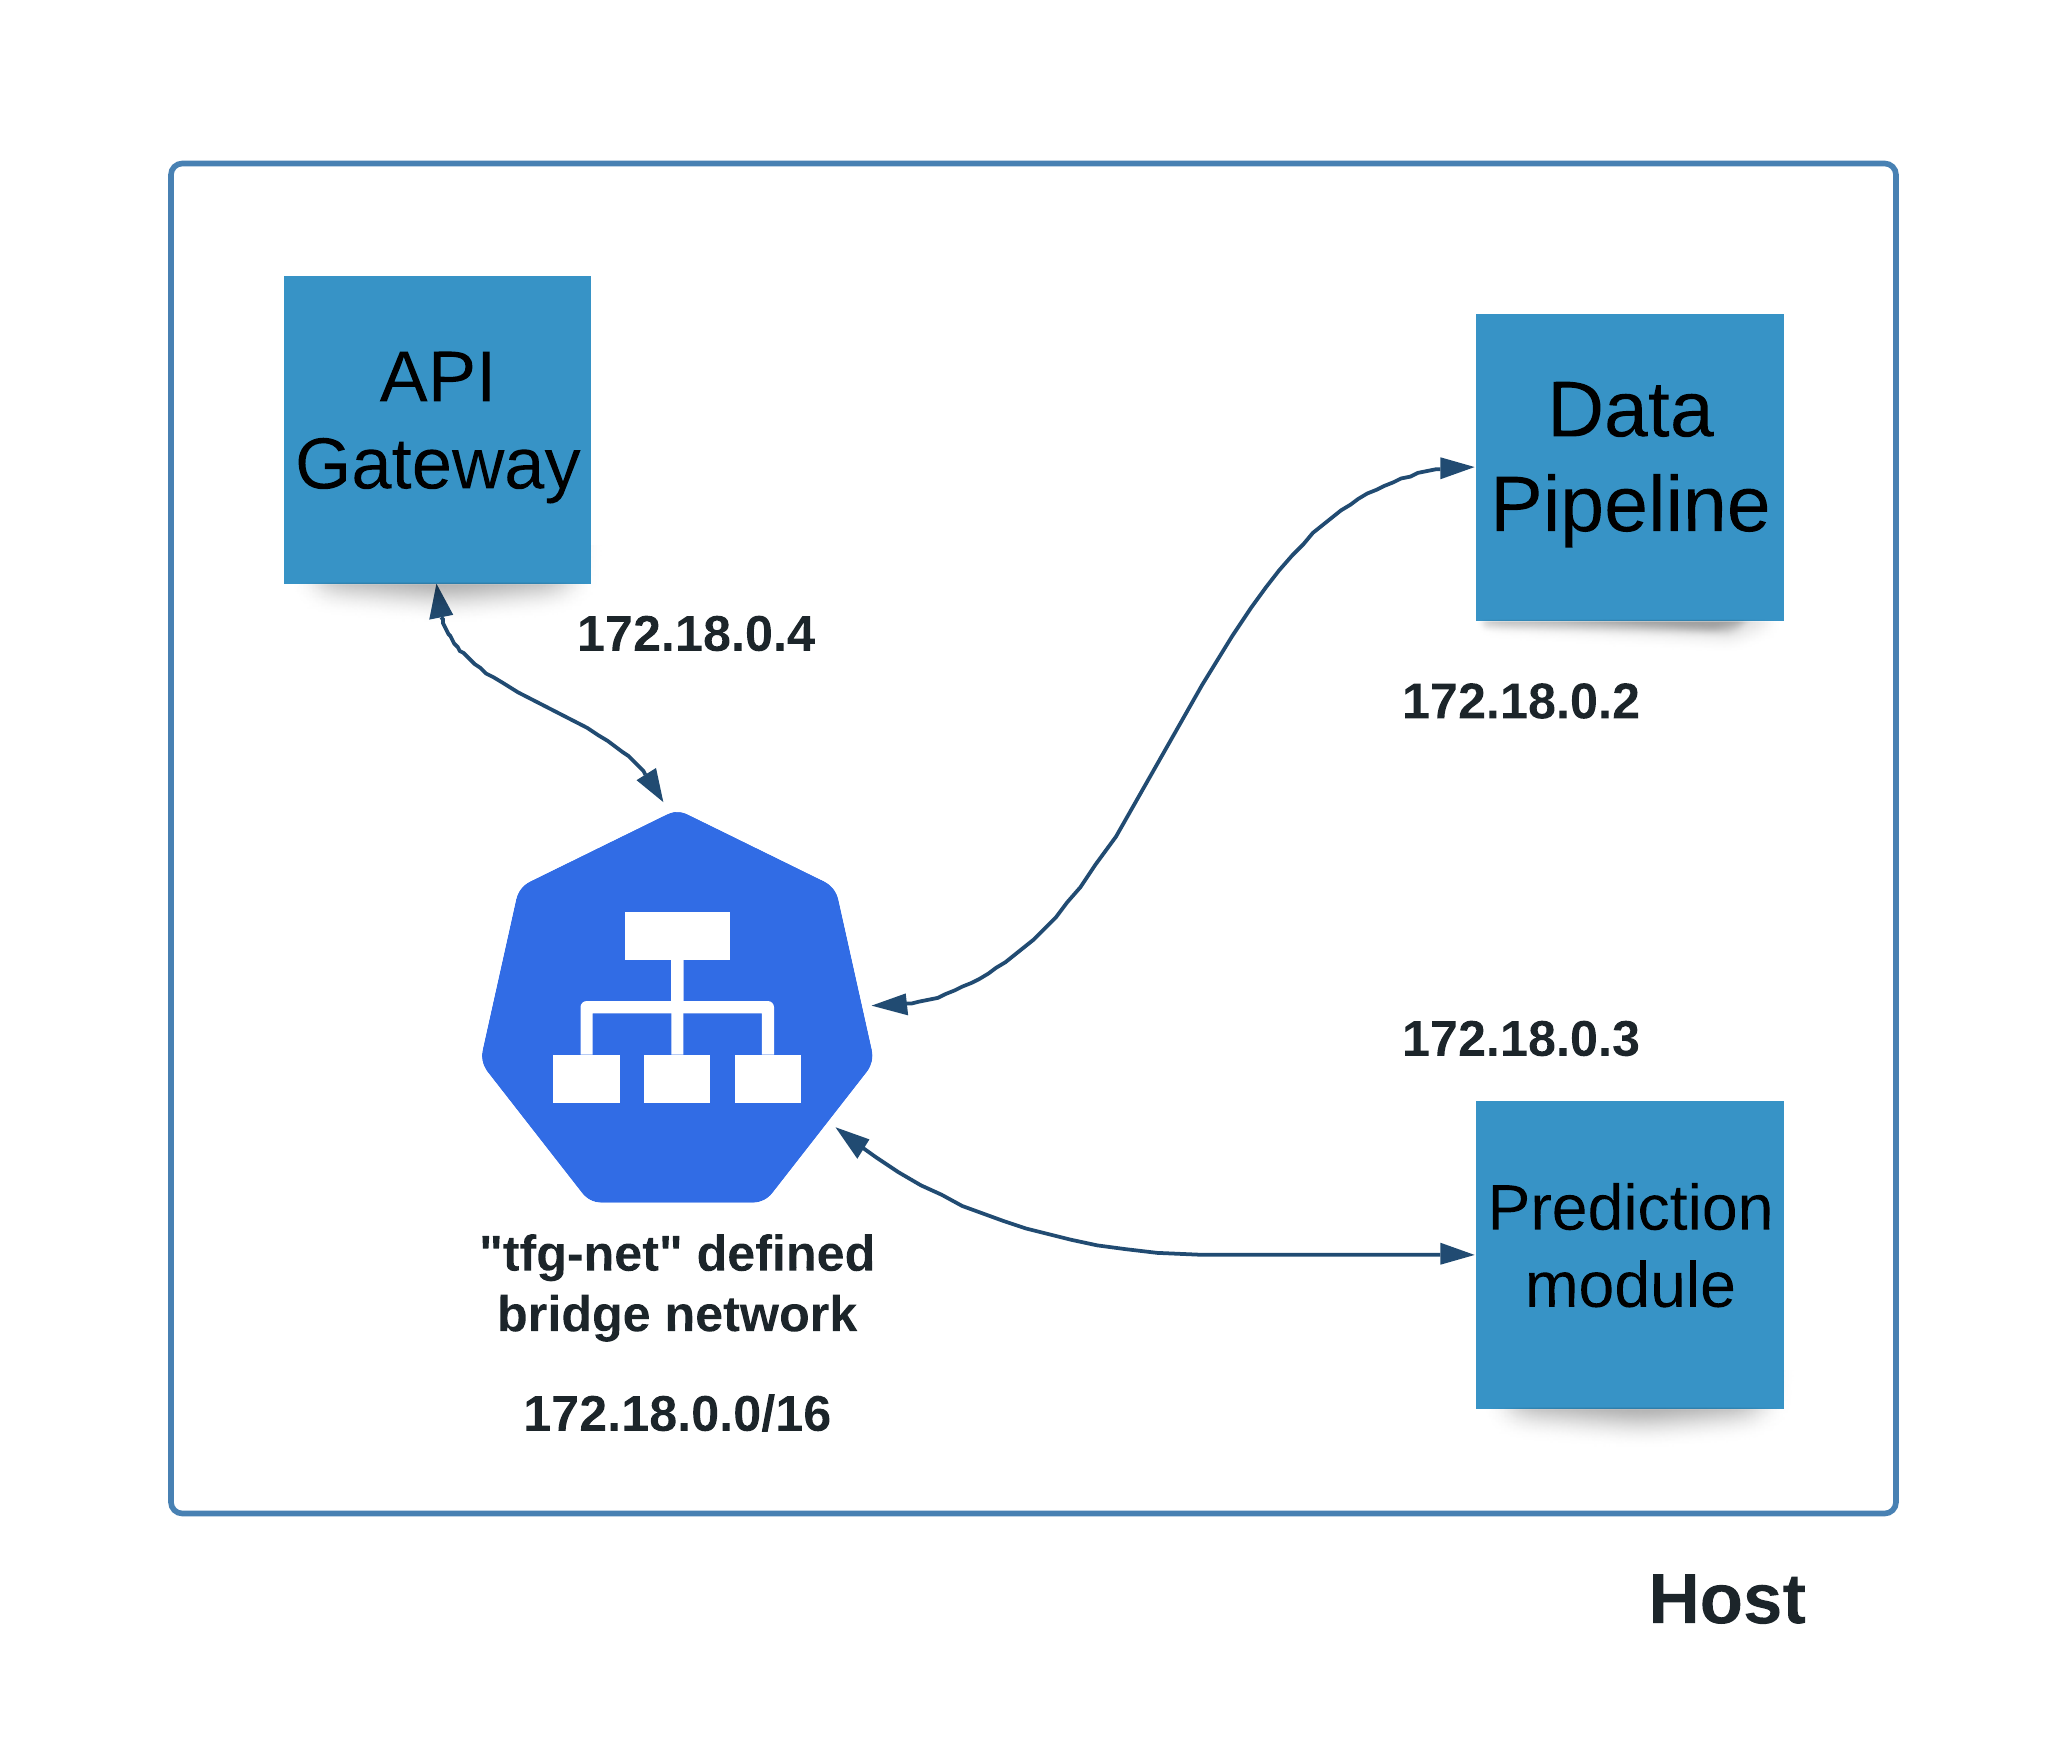
\includegraphics[width=\textwidth]{figures/tfg-net.png}
     \caption{User Defined Network}
    \label{fig:tfg-net}
\end{figure}

Communication will take place between two defined channels, the first one between $"API Gateway \longleftrightarrow Data Pipeline"$ and the second one between $"API Gateway \longleftrightarrow Prediction Module"$. In both scenarios, the Data Pipeline module and the Prediction module act as the server and the \gls{api} Gateway as the client requesting a service. 

Regarding the Python standard library for socket connections, sending data can be achieved with the \lstinline[language=python]{sendall()} function. This function unlike \lstinline[language=python]{send()}, continues to send data until either it all has been sent or an error occurs. None is returned on success. On the other hand, due to packet fragmentation a custom implementation of \lstinline[language=python]{receive()} is needed to make sure all the response data is being received, since the standard library does not support this feature. Listing~\ref{lst:receive-all} shows the custom implementation of \lstinline[language=python]{receiveall()}, notice that all the data sent or received through the socket must be byte encoded.\\

\begin{lstlisting}[language=python,caption=Custom Implementation receiveall(),label={lst:receive-all}]
def receive_all(conn: socket) -> bytes:
    # first we receive a header containing the length of the data
    msg_len = recv_header(conn)
    data = b''
    while len(data) < msg_len:
        packet = conn.recv(msg_len - len(data))
        if not packet:
            break
        data += packet
    return data
\end{lstlisting}

\subsection{API Gateway}

As shown in Figure~\ref{fig:architecture-layout}, the main function of the \gls{api} Gateway is to provide the \gls{RESTful} endpoints users will interact with to obtain their predictions. To satisfy user requests, the Gateway will forward these petitions. First to the Data Pipeline module, which will respond with the historical data of the requested company. Second, after receiving the response It will launch a request to the Prediction module, from which the final price prediction of the requested company will be received. Finally, the \gls{api} Gateway serves the user's original request by returning a \gls{json} file either with the prediction or an error message.

There are several Python frameworks to work with \glspl{api} but \gls{Django} has been the final option due to its market popularity and wide community support, even thought for this project a simpler option like Flask would have been more than enough.

The first step to build our \gls{api} endpoints is to create a new application, which will wrap our micro-service logic, inside our blank Django project in the \textbf{\enquote{projectName/settings.py}} module, as Listing~\ref{lst:settings.py} shows. After creating the application, we need to tell Django to forward all incoming petitions to the newly created app, Listing~\ref{lst:root/urls.py}, as it will take care of all the logic.\newpage

\begin{lstlisting}[language=python,caption=apiGateway/settings.py,label={lst:settings.py}]
# Application definition
INSTALLED_APPS = [
    'django.contrib.admin',
    'django.contrib.auth',
    'django.contrib.contenttypes',
    'django.contrib.sessions',
    'django.contrib.messages',
    'django.contrib.staticfiles',
    'rest_framework', #we add this powerful toolkit for building APIs
    'restApi.apps.RestapiConfig', #points to the restApi config file
]
\end{lstlisting}

\begin{lstlisting}[language=python,caption=apiGateway/urls.py,label={lst:root/urls.py}]
urlpatterns = [
    path('admin/', admin.site.urls),
    # we forward all incoming petitions to the respApi app urls.py module
    path('', include('restApi.urls')) 
]
\end{lstlisting}

\begin{lstlisting}[language=python,caption=restApi/urls.py,label={lst:restApi/urls.py}]
urlpatterns = [
    #forward the petitions to a class based view
    path('prediction/<str:ticker>/', views.PredictionView.as_view()),
]
\end{lstlisting}

Now all petitions are being routed to our application, but we need to specify an endpoint for users to communicate with our service. In Listing~\ref{lst:restApi/urls.py} we create the only endpoint our \gls{api} will recognize, \textbf{\enquote{/prediction/<str:ticker>}}. The last part of the url, \textbf{\enquote{<str:ticker>}}, allows us to serialize the company ticker\footnote{An abbreviation used to uniquely identify publicly traded shares of a particular stock on a particular stock market.}, so that it is passed as a parameter to the corresponding view.

Now that we are capable of routing petitions we need to create a view, which is a Python function or class that takes a web request and returns a web response, to manage them. Two types of views are built-in in the Django framework, function views and class based views, which need to be declared inside the \textbf{\enquote{restApi/views.py}} module. For this project the class based view has been the final option simply because each single \gls{http} request method can be defined by a matching name function, as Listing~\ref{lst:restApi/views.py} shows.

\begin{lstlisting}[language=python,caption=restApi/views.py,label={lst:restApi/views.py}]
class PredictionView(APIView):
    """
    Class based view for all the nasdaq related requests
    """
    def get(self, request, ticker: str):
        client = Client(os.getenv('PIPELINE_IP', 'data-pipeline'), 15032)
        data = client.connect(ticker)
        raw_df = pd.DataFrame(json.loads(data)["Time Series (Daily)"]).T
        for c in raw_df.columns:
            raw_df[c] = pd.to_numeric(raw_df[c])
        raw_df.index = pd.to_datetime(raw_df.index)
        response = requests.post('http://prediction-module:8501/v1/models/{model}:predict', data=json.dumps({
            "signature_name": "serving_default",
            "instances":  raw_df.sort_index().iloc[-1].to_numpy().reshape(1, 5).tolist()
        }))
        return JsonResponse(response.json())
\end{lstlisting}

In section~\ref{Container communication} we explained how containers communicated among one another and that the API Gateway always acted as a client, either to request data to the Data Pipeline module or to the Predcition module as seen in Listing~\ref{lst:restApi/views.py}. Listing~\ref{lst:restApi/client.py} shows the implementation of the client class for communicating with Data Pipeline module using sockets.

\begin{lstlisting}[language=python,caption=restApi/client.py,label={lst:restApi/client.py}]
class Client:
    FORMAT = 'utf-8'
    BUFFER_SIZE = 4096
    HEADER = 64

    def __init__(self, server_ip: str, port: int):
        self.server_ip = server_ip
        self.port = port
        self.server = socket.socket(socket.AF_INET, socket.SOCK_STREAM)

    def connect(self, symbol: str) -> str:
        with self.server as s:
            s.connect((self.server_ip, self.port))
            len_symbol = prepared_send(symbol)
            s.sendall(len_symbol)
            s.sendall(symbol.encode(Client.FORMAT))
            return recv_all(s).decode(Client.FORMAT)

\end{lstlisting}

Last but not least, once we have all the \gls{api} Gateway code implemented, we need to specify \gls{Docker} how to containerize the application so that our build and push workflow in Listing~\ref{lst:build-push-docker} can automatically build and upload the Docker image to Docker Hub. Listing~\ref{lst:ApiGateway-dockerfile} shows the Dockerfile used to create the image to build the container. 


\begin{lstlisting}[language=python,caption=Api Gateway Dockerfile,label={lst:ApiGateway-dockerfile}]
FROM    ubuntu
RUN     apt -y -q update && apt -y -q install python3 python3-pip
COPY    . /api-gateway 
WORKDIR /api-gateway
#install dependencies
RUN     pip3 install -r requirements.txt 
EXPOSE  8000/tcp
ENTRYPOINT ["python3", "manage.py", "runserver", "0.0.0.0:8000"] 
\end{lstlisting}

\subsection{Data pipeline}

\begin{lstlisting}[language=python,caption=aplha-vantage.py,label={lst:alpha-vantage}]
def download_data(symbol: str, function='TIME_SERIES_WEEKLY', dump=False) -> dict:
    valid, best_match = validate_symbol(symbol)
    if not valid:
        return _not_valid(dump)
    url = f'https://www.alphavantage.co/query?function={function}&symbol={best_match}&interval=5min&' \
          F'apikey={API_KEY}'
    r = requests.get(url)
    if dump:
        _dump_data(r.json(), 'api_data.txt')
    return r.json()

def validate_symbol(symbol: str) -> (bool, str):
    url = f'https://www.alphavantage.co/query?function=SYMBOL_SEARCH&keywords={symbol}&apikey={API_KEY}'
    r = requests.get(url)
    matches = r.json().get('bestMatches', None)
    if not matches:
        return False, symbol
    return True, matches[0]['1. symbol']

def _not_valid(dump: bool) -> dict:
    data = {"Error": "No matches found for the requested symbol"}
    if dump:
        _dump_data(data, 'api_data.txt')
    return data

def _dump_data(data: dict, file: str):
    with open(file, 'w') as out:
        json.dump(data, out, sort_keys=True, indent=4)
\end{lstlisting}

The Data Pipeline module's main function, as seen in the architecture layout in Figure~\ref{fig:architecture-layout}, is to wait for petitions, requesting the historical time-series of a given ticker of a company, from the \gls{api} Gateway module. To get the time-series, the Data pipeline module will use the Aplha Vantage \glspl{api}, which provides enterprise-grade financial market data. From traditional asset classes, e.g., stocks and \glspl{etf}, to economic signals, from foreign exchange rates to cryptocurrencies, from fundamental data to technical indicators.~\cite{alphaVantage}

Data from the Alpha Vantage \gls{api} can easily be fetched with the Python package \textbf{\enquote{request}}. Listing~\ref{lst:alpha-vantage} shows the Python implementation to request the data located in the \textbf{\enquote{alpha-vantage.py}} Python module.

In order to be able to respond to requests, we first need to be capable of receiving them. As we mentioned above the Data Pipeline behaves as a server to which the \gls{api} Gateway connects. Listing~\ref{lst:server.py} shows the implementation of the \textbf{\enquote{server.py}} module.

\begin{lstlisting}[language=python,caption=server.py,label={lst:server.py}]
class Server:
    FORMAT = 'utf-8'
    BUFFER_SIZE = 4096
    HEADER = 64

    def __init__(self, addr=None, port=15032):
        if not addr:
            self.addr = socket.gethostbyname(socket.gethostname())
        else:
            self.addr = addr
        self.port = port
        self.server = socket.socket(socket.AF_INET, socket.SOCK_STREAM)

    def start(self):
    """Wait & respond incoming connections"""
        try:
            self.server.bind((self.addr, self.port))
            self.server.listen()
            while True:
                conn, ip = self.server.accept()
                threading.Thread(target=self.manage_client, args=(conn, ip)).start()
        except KeyboardInterrupt:
            self.server.close()

    def manage_client(self, conn: socket, ip: Tuple[str]):
        with conn as c:
            sym_request = recv_all(c).decode(Server.FORMAT)
            self.response_client(sym_request, c)

    def response_client(self, symbol: str, conn: socket):
        data = json.dumps(download_data(symbol))
        encoded_len = prepared_send(data)
        conn.sendall(encoded_len)
        conn.sendall(data.encode(Server.FORMAT))
\end{lstlisting}

As we did in the previous section we need to specify the Dockerfile to build the image. Listing~\ref{lst:dataPipeline-dockerfile} shows the Dockerfile used to create the image to build the container.

\begin{lstlisting}[language=python,caption=Data Pipeline Dockerfile,label={lst:dataPipeline-dockerfile}]
FROM    ubuntu
RUN     apt -y -q update && apt -y -q install python3 python3-pip
COPY    . /alpha-vantage
WORKDIR /alpha-vantage
RUN     mkdir logs
RUN     pip3 install -r requirements.txt
EXPOSE  15032/tcp
ENTRYPOINT ["python3", "main.py"]
\end{lstlisting}

% \notebox{
%     \textbf{"Why do we need to decouple the Data pipeline Module?"}
    
%     After reading this sub-section, you are probably wondering why the Data Pieline module is a container by itself when its logic could just be done inside the \gls{api} Gateway. The main reason besides scalability issues, was to provide a baseline architecture for a future project where more complex data processes  could be applied.
% }

\newpage
\subsection{Prediction module}
\label{prediction-module}

\begin{figure}[h]
    \centering
    \caption{Tensorflow Serving}
    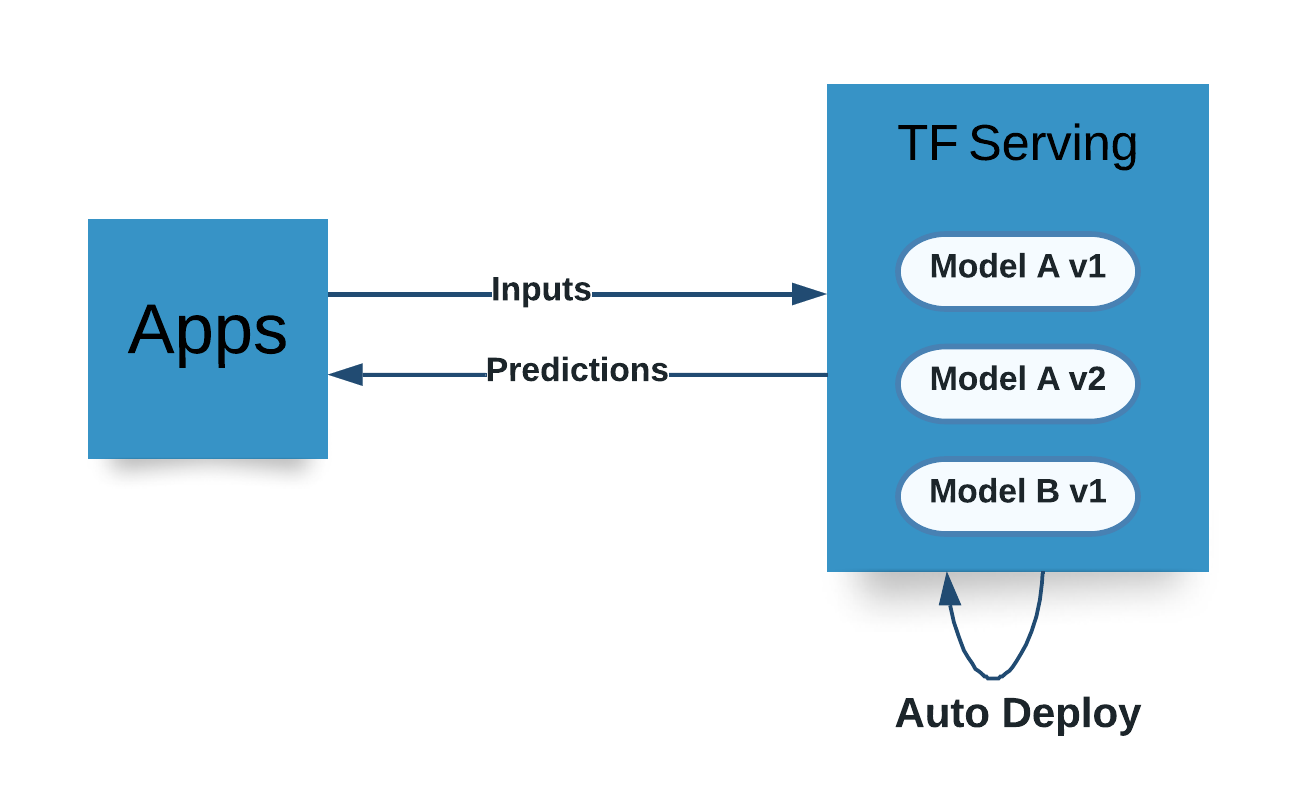
\includegraphics[width=0.8\textwidth]{figures/serving.png}
    \label{fig:serving}
\end{figure}

As introduced in section \ref{Micro-service Architecture} instead of building the micro-service from scratch and reinvent the wheel, we can use Tensorflow Serve. \enquote{A very efficient, battle-tested model server that can sustain a high load, serve multiple versions of your models and watch a model repository to automatically deploy the latest versions}, as Figure~\ref{fig:serving} shows~\cite{handsOnMachine}.

To use this functionality we first need set up some sort of file system structure to save our models and its versions. Using the function \textbf{\enquote{tf.saved\_model.save(model, path)}} we can easily serialize and save our model so it can be loaded by the Tensorflow Serve using the \textbf{\enquote{keras.models.load(model\_path)}} function. Models should be saved under the structure of \enquote{model name} and \enquote{version}, Figure~\ref{fig:model-save}. This will allow the server to auto-deploy all our models and expose them through an \gls{http} or \gls{grpc} endpoint.

\begin{figure}[h]
    \centering
    \caption{Save Keras Model File System Structure}
    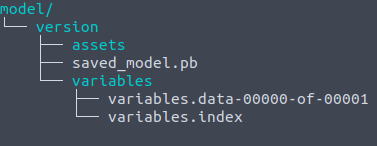
\includegraphics[width=0.75\textwidth]{figures/model-save.png}
    \label{fig:model-save}
\end{figure}

Tensorflow Serve can be easily downloaded from the Tensorflow's official repository. This will allow us to pull the image directly from the orchestrator, Listing~\ref{lst:docker-compose}. We only need to specify the ports which will be used by the REST/gRPC endpoints and mount the folder containing all of our models into our container, so the server knows where to find them. The request made to the http endpoint by the \gls{api} Gateway can be seen in Listing~\ref{lst:restApi/views.py}.

\subsection{Orchestration}

\gls{Docker} compose has been chosen for this project to orchestrate the different containers on the same host. Docker compose is a tool for defining and running multi-container Docker applications. With Compose, you use a \gls{YAML} file to configure your application’s services. Then, with a single command, you build and start all the services from your configuration. Docker compose has the following functionalities for managing the whole life cycle of your application:~\cite{dockerCompose}

\begin{itemize}
    \item Start, stop, and rebuild services.
    \item View the status of running services.
    \item Stream the log output of running services.
    \item Run a one-off command on a service.
\end{itemize}

Listing~\ref{lst:docker-compose} shows the docker compose file used to set up the orchestration configuration. Notice that the \gls{api} Gateway module depends on the other two modules to be initialized. 

\newpage
\begin{lstlisting}[language=python,caption=docker-compose.yaml,label={lst:docker-compose}]
version: "3.9"
services:
        apiGateway:
                image: marcosmartinezfco/tfg-api-gateway
                container_name: api-gateway
                networks:
                        - tfg-net
                ports:
                        - "8000:8000"
                depends_on:
                        - dataPipeline
        dataPipeline:
                image: marcosmartinezfco/tfg-data-pipeline
                container_name: data-pipeline
                networks:
                        - tfg-net
        predictionModule:
                image: tensorflow/serving
                container_name: prediction-module
                networks:
                        - tfg-net
                ports:
                        - "8501:8501"
                depends_on:
                        - dataPipeline
                volumes:
                        - ${MODELPATH}/mlp_model:/models/mlp_model
                environment:
                        - MODEL_NAME=mlp_model
networks:
        tfg-net:
                name: tfg-net
                driver: bridge
\end{lstlisting}

\section{Neural Network Definition}
\label{NN definition}

A key aspect of some types of \gls{ann} such as densely connected networks is that they have no memory. They process each input independently, without recording any state in between inputs. In contrast, as you are reading the present sentence, you are processing it word by word, while keeping memories of what came before\cite{deepWithPython}.

This lack of memory may present issues with any type of data that is time related or needs to keep a record of its past. \glspl{rnn} tackle this problem by iterating through the sequence elements and maintaining a state containing information relative to what it has seen so far. In essence, a \gls{rnn} is a type of \gls{ann} with an internal loop.

In this section we will walk through the development of a model capable of making predictions on stock prices using the historical time series of its price. But before trying to implement the model, we need to understand the problem, so that the whole process is easier. The following aspects need to be considered:

\begin{itemize}
    \item Understand what we are trying to predict and its business logic.
    \item Identify the type of problem we are dealing with.
    \item Define what and how to process the data.
\end{itemize}

It is obvious we are facing a regression problem since we are trying to predict a numeric value, the price. In regards to the business logic, we talked in section \ref{SoA:estado del arte} about how different features may have and impact on an asset's price. Along this chapter we will find out whether is possible to obtain good predictions just based on the past prices of an asset or if more features are needed to be taken into account.

\subsection{Data definition}

During the whole training process, only the historical data of Google will be used in the training for simplicity's sake. This data will be presented as a time series, as shown in Figure~\ref{fig:training-data}, containing the weekly or daily trading (depending of sample size requirements) information, i.e, the open price, close price, highest trading price, lowest trading price and the trading volume in dollars.

\begin{figure}[H]
    \centering
    \caption{Weekly Time Series of Google}
    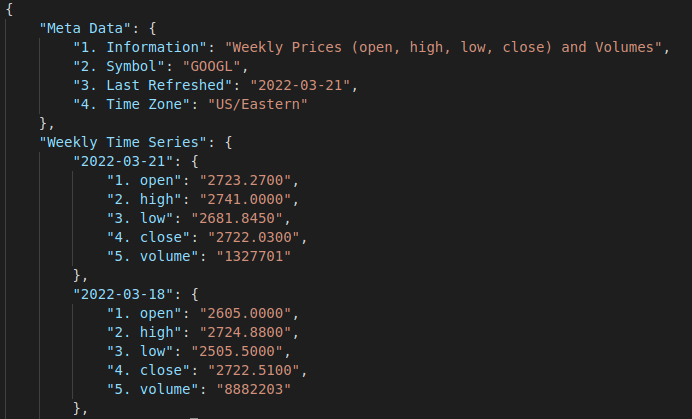
\includegraphics[width=0.8\textwidth]{figures/train data.png}
    \label{fig:training-data}
\end{figure}

Now we can easily transform our \gls{json} into a pandas data frame to easily manage information. Listing~\ref{lst:load-data} shows how to load the \gls{json} into our data frame with the date time as our index.

\begin{lstlisting}[language=python,caption=Load Data Into a Pandas Data Frame,label={lst:load-data}]
with open('./Training data/googl.json') as f:
    data = json.load(f)
raw_df = pd.DataFrame(data["Weekly Time Series"]).T
raw_df = raw_df.rename(lambda x: x.split(' ')[1], axis=1)
for c in raw_df.columns:
    raw_df[c] = pd.to_numeric(raw_df[c])
raw_df.index = pd.to_datetime(raw_df.index)
raw_df = raw_df.sort_index()
\end{lstlisting}

\subsection{Simple Interpolation Approach}

Now that we have all our training data prepared we can move on to the next step in the process, which is creating a basic model without artificial intelligence. It will give us a baseline point from which we can evaluate the most basic solution and why it may be interesting to use \gls{ai} algorithms.

\begin{lstlisting}[language=python,caption=Price Extrapolation,label={lst:base-model}]
def simple_predictions(df):
    success = 0
    forecast = []
    for x in range(3, len(df)-1):
        interpolate = interp1d(range(4), [(df.iloc[row]['open'] + df.iloc[row]['close']) / 2 for row in range(x-3, x+1)], kind='slinear', fill_value='extrapolate', bounds_error=False)
        forecast.append(t:=interpolate(4))
        if  df.iloc[x+1]['open'] <= t <= df.iloc[x+1]['close'] or df.iloc[x+1]['open'] >= t >= df.iloc[x+1]['close']:
            success += 1
    print(f'accuracy {success/(len(df)-4)*100}%')
\end{lstlisting}

We will build a prediction algorithm which will take into consideration the prices of the asset over the last month and its price trend, as Figure~\ref{fig:price-trend} shows, and interpolate a prediction linearly proportional to the trend. Listing~\ref{lst:base-model} shows a simple function that computes and test this approach, reaching 33.69\% accuracy in the whole data frame, Figure~\ref{fig:basic-acurracy} shows the accuracy for the last 40 weeks.

\begin{figure}[H]
    \centering
    \caption{Basic Price Trend}
    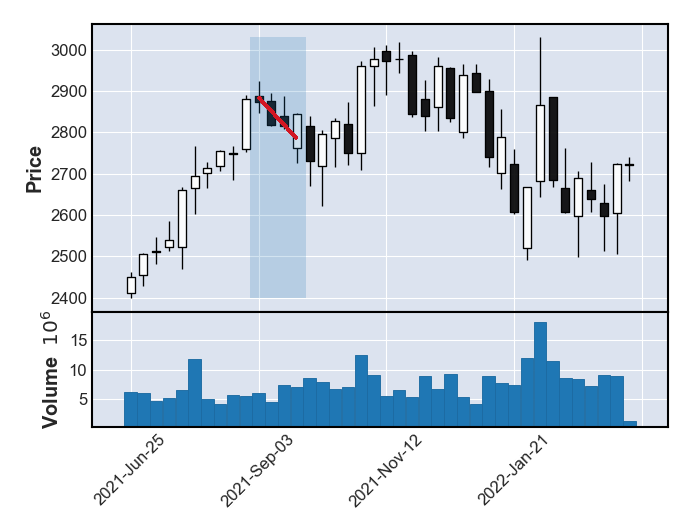
\includegraphics[width=0.7\textwidth]{figures/baselineCalc.png}
    \label{fig:price-trend}
\end{figure}

\begin{figure}[H]
    \centering
    \caption{Basic Model Accuracy, Last 40 Weeks}
    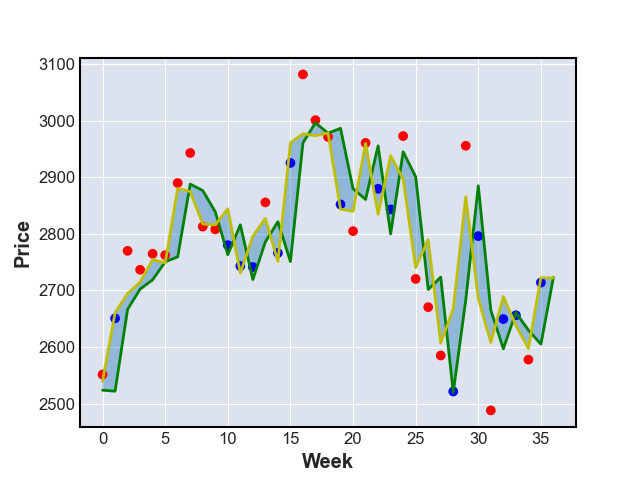
\includegraphics[width=0.7\textwidth]{figures/simple.png}
    \label{fig:basic-acurracy}
\end{figure}

\subsection{Multilayer Perceptron Approach}

Once we have a baseline model, let's find out if we can improve the prediction accuracy with a simple \gls{mlp}. Due to the small sample size of the weekly time series, daily time series data will be used for the deep learning algorithms instead. Listing~\ref{lst:perceptron} shows the assembly of the network. Figure~\ref{fig:perceptron} shows the accuracy obtained by the model in the test data set, reaching 31\%

\begin{lstlisting}[language=python,caption=\gls{mlp} Assembly,label={lst:perceptron}]
inputs = keras.Input(shape=(5,))
x = keras.layers.Dense(5, activation="relu")(inputs)
x = keras.layers.Dense(6, activation="relu")(x)
x = keras.layers.Dense(3, activation="relu")(x)
output = keras.layers.Dense(1, activation="linear")(x)
model = keras.Model(inputs=inputs, outputs=output, name="MLP")
model.compile(
    loss=keras.losses.MeanSquaredError(),
     optimizer=keras.optimizers.Adam(learning_rate=0.00001),
)
\end{lstlisting}

\begin{figure}[H]
    \centering
    \caption{\gls{mlp} Accuracy Over the Last 100 Days}
    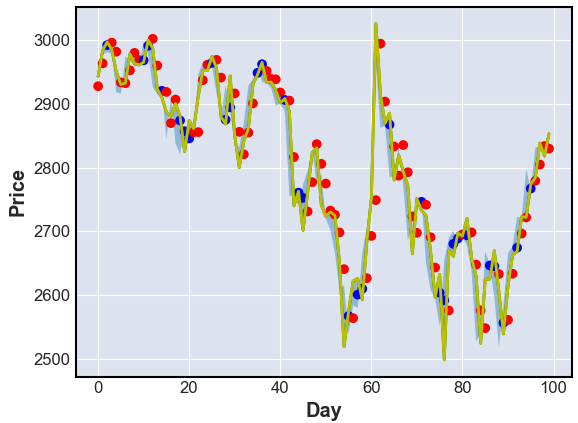
\includegraphics[width=0.7\textwidth]{figures/mlp.png}
    \label{fig:perceptron}
\end{figure}

After multiple hyper-parameter tunings~\footnote{\url{https://xkcd.com/1838/}}, it has been quite normal for the model to overfit and ending up giving the same prediction regardless of the input value. The final conclusion is that the model is unable to learn any correlation in price, given the input features, due to its simplicity. It tried to learn an average value for which the loss could be minimized rather than trying to recognize patterns in the data. That same value it was giving repeatedly could be that average value.

\subsection{Recurrent Neural Network Approach}

In section \ref{Artificial Intelligence} we talked about how \glspl{rnn} can keep an internal state and remember patterns inside our data. We will try now to build a simple model to see if we can improve the lack of memory seen in previous approaches.

First we need to prepare the information we are going to feed to the model. The weekly trading history of GOOGLE contains less than 800 samples which is quite little information. To solve this problem we take the daily trading history of the company and squeeze the data into weeks, Listing~\ref{lst:time-steps}, so now we have around 800 samples with 5 time steps each, shape (786,5,5) at the time of writing.

\begin{lstlisting}[language=python,caption=Week Time Steps GOOGLE,label={lst:time-steps}]
def week_batch_generator(raw, scaler):
    raw_df = scaler.transform(raw)
    df_x = raw_df[:-1]
    df_y = np.array([(x[0]+x[3])/2 for x in raw_df[1:]])
    x_batch = df_x[:-(len(df)%5)].reshape((len(df_x)//5, 5, 5)) 
    y_batch = df_y[:-(len(df)%5)].reshape(len(df_y)//5, 5, -1)
    return (x_batch[:-100], y_batch[:-100]), (x_batch[-100:], np.array(raw_df[1:-(len(df)%5),[0, 3]][-100:]))
\end{lstlisting}

During training we have used two different callbacks. These are objects that can perform actions at various stages of training, e.g, at the start or end of an epoch or before or after a single batch. First, we have the \textbf{\enquote{EarlyStopping}} class which allows to stop training when a given metric shows no improvement, like training loss in this particular case. Second, we have implemented a custom callback class which allows to see graphic representation of the training and validation loss during in real time during training, Listing~\ref{lst:callback}. These callbacks are added to the network configuration as shown in Listing~\ref{lst:lstm-assembly}.

\begin{lstlisting}[language=python,caption=Custom Keras Callback,label={lst:callback}]
Created with the help of Rubén Rincón Blanco
class MyCallback(keras.callbacks.Callback):
    def on_epoch_end(self, epoch, logs = None):
        plt.rcParams["figure.figsize"] = (30,10)
        fig, ax = plt.subplots()
        fig.suptitle(f"epoch: {epoch}, {logs}")
        history = list(logs.keys())
        for key in history:
            if key not in self.valores:
                self.valores[key] = []
            self.valores[key].append(logs[key])
            ax.plot(self.valores[key], label = key, c = colors[0 if "loss" in key else 1], linestyle='--' if 'val' in key else '-')
            ax.legend(loc = "upper right" if "loss" in key else "upper left")
        plt.show()
        display.clear_output(wait = True)
    def __init__(self):
        self.valores = {}
    def on_train_end(self, logs = None):
        print(f"Finished: {logs}")
\end{lstlisting}

\begin{lstlisting}[language=python,caption=\gls{lstm} Assembly,label={lst:lstm-assembly}]
inputs = keras.layers.Input(shape=(x_train.shape[1:]))
x = keras.layers.LSTM(3, activation=keras.layers.LeakyReLU() , return_sequences=True)(inputs)
x = keras.layers.Dropout(0.2)(x)
x = keras.layers.LSTM(2, activation=keras.layers.LeakyReLU() , return_sequences=False)(x)
x = keras.layers.Dropout(0.2)(x)
output = keras.layers.Dense(1, activation='linear')(x)
model_lstm = keras.Model(inputs=inputs, outputs=output, name="v1.0")
model_lstm.compile(
    loss=keras.losses.MeanSquaredError(),
    optimizer=keras.optimizers.Adam(learning_rate=0.00001),
)
history = model_lstm.fit(
    x_train[:-100], y_train[:-100],
    validation_data=(x_train[-100:], y_train[-100:]), 
    batch_size=32, epochs=100, shuffle=False,
    verbose=0,
    callbacks=[
        keras.callbacks.EarlyStopping(patience=15, restore_best_weights=True),
        MyCallback()
    ]
)
\end{lstlisting}

\begin{figure}
    \centering
    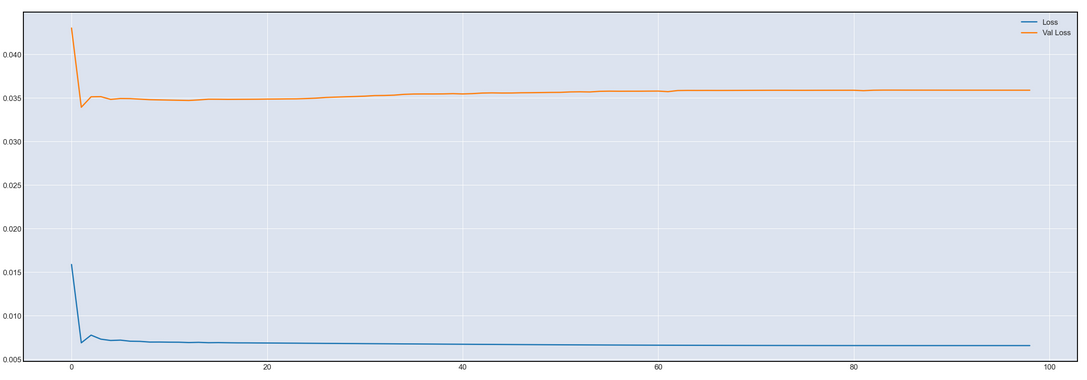
\includegraphics[width=\textwidth]{figures/loss-lstm.png}
    \caption{\gls{lstm} Training Loss}
    \label{fig:loss-lstm}
\end{figure}

As in the previous section, the \gls{lstm} model presents high levels of overfitting, Figure~\ref{fig:loss-lstm} . It also presents huge sings of mode collapse\footnote{When model can only produce a single type of output or a small set of outputs regardless of the input data.} within the average price range of the trading history, as seen with the \gls{mlp} model, regardless of the hyper-parameters configuration. 



\chapter{Results}
\label{res:resultados}

Stock price forecasting is an interesting field of application of \gls{ai} given the intrinsic correlation between statistics and financial markets. Computers are extremely efficient at recognizing patterns, thus they can identify price trends and patterns that may be embedded in in an asset's price history. Nonetheless, as we discussed in the introduction section \ref{ch:introduccion}, it is a naive approach to believe that the future can be entirely predicted based on the past. Multiple conjoined factors all together, some of which may be variable, drive the price of an asset.

This hypothesis is backed by the results obtained during the development of section \ref{NN definition} where both the \gls{mlp} model and the \gls{lstm} model presented high levels of overfitting and mode collapse around the overall average price range of the trading history of GOOGLE. The first one had a better performance overall and didn't present as much mode collapse whereas the \gls{lstm} network didn´t made any learning no matter what configuration or regularization was applied. In the end the interpolation approach, which was intended to be the baseline model, ended up being the one with the highest accuracy whereas the \glspl{ann} struggled to learn meaningful patterns in the price history of GOOGLE. Better training processes and more meaningful, complete and price-relevant market information would be needed.

Regarding deployment, during section \ref{SoA:estado del arte} we discovered how the microservices architecture along with containerization techniques can establish a highly scalable architectural pattern. Throughout the entire thesis we have focused on merging these two technologies to get an overall understanding. However, there is one key concept you may have noticed which has not been the main focus during development, concurrency. Concurrency is a extremely important aspect since all the advantages provided by our architecture can not be fully exploited without it. Although some parts of the architecture support concurrency, like the prediction module \ref{prediction-module}, other parts such as the socket communication protocol between the \gls{api} Gateway and the Data Pipeline modules make use of blocking methods, restricting throughput. Nonetheless, the use of technologies such as Docker, the microservices pattern and \gls{cd} strategies have made it possible to set up a development environment with an extremely low delay between code and deployment with almost every process being automated.

\chapter{Conclusions}
\label{con:conclusions}
\section{Social Impact}
\label{imp:impacto}

Being able to imagine \gls{ai}'s monstrous magnitude of power, can we assert whether or not it will do good to society? There is a lot of controversy around this question and arguments can be found on both sides.

Throughout history it has been clear that mankind always looks for tools to finish tasks faster, easier, more effectively, and more conveniently. Thus, \gls{ai} has also managed to find and stay in a spot for the last decade~\cite{tai2020impact}.

There is a possible dark side to what \gls{ai} may provide humanity economically speaking. There may come a time when human labor will no longer be needed as everything can be done mechanically. Humanity will need to adapt, for example by taking care of inherently human tasks, i.e, tasks related with empathy, emotions or those that are socially oriented. Nevertheless, some people like Elon Musk, with a more optimistic approach to the growth of \gls{ai}, believe there is a pretty good chance we end up with a universal basic income, due to automation~\cite{elonBasicIncome}. In contrast, there are other more pessimistic figurehead that envision a dystopic future lead by machine minds rather than human hearts.

On the other side, there are several areas where \gls{ai} can have a predictable positive impact such as healthcare, where it can provide multiple benefits: a) Faster and more accurate diagnostics ;b) Reduce errors related to human fatigue ; c) Improved radiology; d) Socially therapeutic robots.

Hence, regarding the social impact on financial markets, \gls{ai} can establish a thriving development framework for economic growth given its ease at recognizing patterns. Nonetheless, this can also become a drawback since inequality could be created as investors can end up taking the major share of the earnings, widening the gap between the rich and the poor.

\section{Future Lines of Work}
\label{fu:future}

During the development phase of the thesis some aspects were discussed in a brief manner, since providing a deeper insight would be the subject of a whole thesis, thus falling outside the scope proposed for this paper.

One of the facets that could be expanded is the micro-service architecture, which we talked about in section \ref{Micro-services Architecture}. We explained the main advantages this pattern could offer in terms of scalability and throughput. One line of work would be to focus on concurrency and performance scaling.

Similarly, orchestration is another key point that could be further developed. For simplicity reasons, Docker compose has been used which means that all containers run on the same host machine. One line of work would be to explore other orchestration tools and techniques such as Kubernetes, and make use of cloud computing and auto-scaling processes to maximize availability and scalability.

Finally, the prediction module is one, if not the most, important component since it is responsible of providing the predictions. Throughout the entire thesis we have compared multiple approaches and encountered multiple difficulties. One line of work would be to develop more complex models putting special attention on the training data. More parameters could be included as part of the information to feed the models, since the stock market is influenced by multiple factors as pointed in section \ref{ch:introduccion}.

\printbibliography
\clearpage
\printglossaries

\end{document}
